\def\qI{\ensuremath{\mathcal{I}}}
\def\TT{\ensuremath{\mathrm{TT}}}
\def\fGW{\ensuremath{f_{\mathrm{GW}}}}

In this chapter we briefly review the theory of gravitational waves: how they arise in \ac{GR} and how they can be detected by an interferometer. We then review the physics behind the \ac{LIGO} and Virgo interferometers, including their main sources of noise. Finally, we examine potential sources of \ac{GW} waves that can be detected by the \ac{LIGO} and Virgo interferometers.

\section{Gravitational Waves in General Relativity}
\label{sec:gr}

In this section we show how gravitational-waves arise in General Relativity. We begin our discussion with Einstein's field equations, given by\footnote{We will work in ``natural units" in which $G = c = 1$, where $G$ is Newton's gravitational constant and $c$ is the speed of light.} \cite{ref:Einstein}:
\begin{equation}
\label{eqn:einstein_field_eqns}
G_{\alpha\beta} = 8\pi T_{\alpha \beta}
\end{equation}
where $T_{\alpha\beta}$ is the stress-energy tensor and $G_{\alpha\beta}$ is the Einstein curvature tensor, defined as:
\begin{equation}
G_{\alpha\beta} \equiv R_{\alpha \beta} - \frac{1}{2}R g_{\alpha\beta}
\end{equation}
Here, $g_{\alpha\beta}$ is the metric on some manifold and $R$ is the Rici curvature scalar, which is obtained by contracting $R_{\alpha\beta}$, which is the Rici tensor. The Rici tensor is obtained by contracting the Riemann curvature tensor, $R\indices{^\alpha_{\beta\mu\nu}}$, on the first and third indices. Riemann is defined as:
\begin{equation}
R\indices{^\alpha_{\beta\mu\nu}} \equiv \Gamma\indices{^\alpha_{\beta\nu,\mu}} - \Gamma\indices{^\alpha_{\beta\mu,\nu}} + \Gamma\indices{^\alpha_{\sigma\mu}}\Gamma\indices{^\sigma_{\beta\nu}} - \Gamma\indices{^\alpha_{\sigma\nu}}\Gamma\indices{^\sigma_{\beta\mu}}
\end{equation}
where the $\Gamma\indices{^\alpha_{\mu\nu}}$ are the Christoffel symbols, given by:
\begin{equation}
\Gamma\indices{^\alpha_{\mu\nu}} = \frac{1}{2}g^{\alpha\beta}(g_{\beta\mu,\nu} + g_{\beta\nu,\mu} - g_{\mu\nu,\beta})
\end{equation}
The ``," indicates the partial derivative of the tensor with respect to the trailing indices. The Christoffel symbols give the change in the metric as it is moved along a path in a curved manifold. Stepping back up the ladder, the Riemann tensor gives the change in the metric when we go around a small closed path. It thereby describes the curvature of the manifold, in $20$ independent components (in a four-dimensional spacetime). The Rici tensor reduces the number of components to $10$, and the Einstein tensor to $6$, leaving $4$ components of the metric free \cite{ref:BlanfordThorne}.\footnote{These four free components allow us to choose any coordinate system, or ``gauge", we wish without changing the underlying physics.} Thus the Einstein field equations relate the curvature of spacetime to mass and energy, which gives rise to the ``force" we call gravity. (Voil\`{a}. \ac{GR} in a nutshell.)

In a strongly curved spacetime, the full Einstein field equations cannot be solved analytically. We will therefore concern ourselves with the weak field limit, in which:
\begin{align}
g_{\alpha\beta} = \eta_{\alpha\beta} + h_{\alpha\beta}
\end{align}
Here, $\eta_{\alpha\beta}$ is the Minkowski metric (we use the $(-,+,+,+)$ convention) and $h_{\alpha\beta}$ is a small perturbation on this metric, i.e., $|h_{\alpha\beta}| \ll 1$. With this assumption, the Riemann tensor simplifies to \cite{ref:Schutz}:
\begin{equation}
R\indices{_{\alpha\beta\mu\nu}} = \frac{1}{2}(h_{\alpha\nu,\beta\mu} + h_{\beta\mu,\alpha\nu} - h_{\alpha\mu,\beta\nu} - h_{\beta\nu,\alpha\mu})
\end{equation}
If we define $\bar{h}^{\alpha\beta}$ to be the ``trace reverse" of $h_{\alpha\beta}$:
\begin{equation}
\bar{h}_{\alpha\beta} = h_{\alpha\beta} - \frac{1}{2}\eta_{\alpha\beta}h
\end{equation}
(here $h = h\indices{^\sigma_\sigma}$ is the trace of h) then, to first order, we can simplify the Einstein curvature tensor to:
\begin{equation}
G_{\alpha\beta} = -\frac{1}{2}(\bar{h}\indices{_{\alpha\beta,\mu}^\mu} + \eta_{\alpha\beta}\bar{h}\indices{_{\mu\nu}^{,\mu\nu}} - \bar{h}\indices{_{\alpha\mu,\beta}^\mu} - \bar{h}\indices{_{\beta\mu,\alpha}^\mu} + \mathcal{O}(h^2_{\alpha\beta}))
\end{equation}
We can exploit gauge freedoms in the Einstein equations to simplify this more. If we chose the Lorenz gauge,
\begin{equation}
\bar{h}\indices{^{\mu\nu}_{,\nu}} = 0
\end{equation}
then:
\begin{equation}
G_{\alpha\beta} = -\frac{1}{2}\bar{h}\indices{_{\alpha\beta,\mu}^\mu}
\end{equation}
The weak-field Einstein equations are thus:
\begin{equation}
\label{eqn:wave_eqn}
\Box\bar{h}_{\alpha\beta} = -16\pi T_{\alpha\beta}
\end{equation}
where $\Box$ is the d'Almbertian operator. This is the wave equation. Analogous to the wave equation in electromagnetism, equation \ref{eqn:wave_eqn} has the solution:
\begin{equation}
\label{eqn:wave_sol-source}
\bar{h}_{\alpha\beta} = 4 \int \frac{T_{\alpha\beta}(t - |\vec{x}-\vec{x}'|, \vec{x}')}{|\vec{x} - \vec{x'}|} \d x'^3
\end{equation}

Equation \ref{eqn:wave_sol-source} relates the metric pertubation to its source. We will return to this equation shortly. First, to explore properties of \ac{GW} propagation, we consider the field equations at points outside the source, i.e., in vacuum, for which $T_{\alpha\beta} = 0$. The wave equation becomes:
\begin{equation}
\Box\bar{h}_{\alpha\beta} = 0
\end{equation}
which has the solution:
\begin{equation}
\label{eqn:wave_sol-vac}
\bar{h}_{\alpha\beta} = \Re A_{\alpha\beta} e^{ik_\mu x^\mu}
\end{equation}
Each $\alpha\beta$ component of $\Bar{h}$ is thus a sinusodial wave that travles along the vector $k^\mu$ with amplitude $A_{\alpha\beta}$. It can be shown \cite{ref:Schutz} that $k_\mu k^\mu = 0$, i.e., $k^\mu$ is a null vector. Identifying $k^0$ as the angular frequency of the wave, $\omega$, this implies that  $|\vec{k}|^2 = \omega^2$. Since, in general, $|\vec{k}| = \omega/v$ (where $v$ is the phase velocity of the wave), $v$ (as well as the group velocity) must be 1. The wave therefore travels at the speed of light. Additionally, in the Lorenz gauge:
\begin{equation}
\label{eqn:lorenz_cond_wave}
A_{\alpha\beta}k^\beta = 0
\end{equation}
This means that $A_{\alpha\beta}$ must be orthogonal to $\vec{k}$; i.e., the wave is a transverse-plane wave.

We can exploit additional gauge freedoms to further simplify the wave equations \ref{eqn:wave_sol-vac}. It can be shown \cite{ref:Schutz} that we can impose two further conditions:
\begin{align}
A\indices{_{\alpha}^{\alpha}} = 0 \\
A_{\alpha\beta}u^{\beta} = 0
\end{align}
while still satisfying the Lorenz gauge condition. The first makes $\Bar{h}_{\alpha\beta}$ trace free; thus in this gauge, which we denote by a TT superscript (the reason for which will become clear shortly),
\begin{equation}
\Bar{h}^{\TT}_{\alpha\beta} = h^{\TT}_{\alpha\beta}
\end{equation}
The second condition sets the $\alpha$ component of $A$ orthogonal to some constant four-velocity of our choosing. If we orient our background reference frame such that the four-velocity lies along the time basis vector, $u^\beta = \delta\indices{^{\beta}_0}$, and such that the spatial part of the wave-vector points along the $z$-axis (i.e, $k = (\omega,0,0,\omega)$) then this condition implies that $A_{\alpha0}$ and $A_{\alpha z}$ are $0$ for all $\alpha$. (The second result follows from equation \ref{eqn:lorenz_cond_wave}.) Thus in this gauge, the metric pertubation is both transverse and traceless, hence the TT label.

By going to the TT gauge we have greatly simplied the solution to the wave equation. Since the metric perturbation is transverse, the only non-zero elements are $h^\TT_{xx}$, $h^\TT_{yy}$, and $h^\TT_{xy}$ (= $h^\TT_{yx}$). Since it is traceless, $h^\TT_{xx} = -h^\TT_{yy}$. Thus we have reduced solutions \ref{eqn:wave_sol-vac} to two independent equations:
\begin{align}
h^\TT_{xx} = \Re h_\pls e^{ik_\mu x^\mu} = h_\pls \cos(\omega(t-z) + \phi_0) \\
h^\TT_{xy} = \Re h_\crs e^{ik_\mu x^\mu} = h_\crs \cos(\omega(t-z) + \phi_0)
\end{align}
where $h_\pls$ ($= A_{xx} = -A_{yy}$) and $h_\crs$ ($= A_{xy} = A_{yx}$) are the ``plus" and ``cross" polarizations of the gravitational wave. ($\phi_0$ is some arbitrary initial phase.)

Since we have used all of our gauge freedoms to obtain these two solutions, the results are physically observable. We can see this by considering the proper distance between two freely-falling particles, one located at the origin ($x_1^i = (0,0,0)$) and the other at $x_2^i = (\delta x,0,0)$ when a gravitational wave passes by. In Cartesian coordinates the line element in the TT gauge is:
\begin{align*}
\d s^2 &= -\d t^2 + \d z^2 + (1+ h_\pls \cos(\omega[t-z]+\phi_0)) \d x^2 \\
     &+ (1 - h_\pls \cos(\omega[t-z]+\phi_0)) \d y^2 + 2 h_\crs \cos(\omega[t-z]+\phi_0) \d x \d y
\end{align*}
To get a sense of the effect of the passing wave, consider the case when the wave only has plus polarization. Additionally, let the initial phase of the gravitational wave be $\phi_0 = -\pi/4$. The proper distance between the two particles at arbitrary time $t$ is: 
\begin{align}
\Delta l = \int \d s &= \int_0^{\delta x} \sqrt{(1 + h_\pls \cos(\omega t - \pi/4))} \d x \\
    &\approx \int_0^{\delta x} (1 + \frac{1}{2} h_\pls \cos(\omega t - \pi/4)) \d x \\
    &= \delta x (1 + \frac{1}{2} h_\pls \cos(\omega t - \pi/4))
\end{align}
In the second step we have used the fact that $|h_\pls| \ll 1$. At time $t=0$, we get $\Delta l = \delta x$, as expected. At time $t= \pi/4\omega$, however, we get $\Delta l = \delta x(1 + h_\pls/2)$: the particle has moved from the origin by an additional $h_\pls/2$. If we perform the same analysis for another particle situated at $x_3^i = (0,\delta y, 0)$, we will get $\Delta l = \delta y(1 - h_\pls/2)$ at time $t = \pi/4\omega$. Likewise, if we consider particles situated at $x^i = (\delta x, \delta y, 0)$ and $x^i = (-\delta x, \delta y, 0)$ we will get similar oscillations when a cross-polarized wave passes through. Figure \ref{fig:hpls-hcrs} shows what this would look like for a ring of particles. Thus, we can detect a gravitational wave by measuring how the proper distance changes between two freely-falling masses. How this is done is explained in section \ref{sec:interferometry}.

Return now to the source-dependent wave solution, equation \ref{eqn:wave_sol-source}. Since the TT gauge captures all of the physically measureable quantities of the gravitational wave outside the source, we can simplify the equation to:
\begin{equation}
\label{eqn:wave_from_source}
h^\TT_{ij} = 4 \left[\int \frac{ T_{ij}(t - |\vec{x}-\vec{x}'|, \vec{x}')}{|\vec{x} - \vec{x'}|} \d x'^3\right]^\TT
\end{equation}
In other words, we can calculate the measureable gravitational wave created by a source from the $ij$ components of the stress-energy tensor alone. We then throw out the transverse parts and remove the trace. We will use this result in the next section to find a solution for the gravitational waveform from a compact binary system.

\begin{figure}[htb]
\center
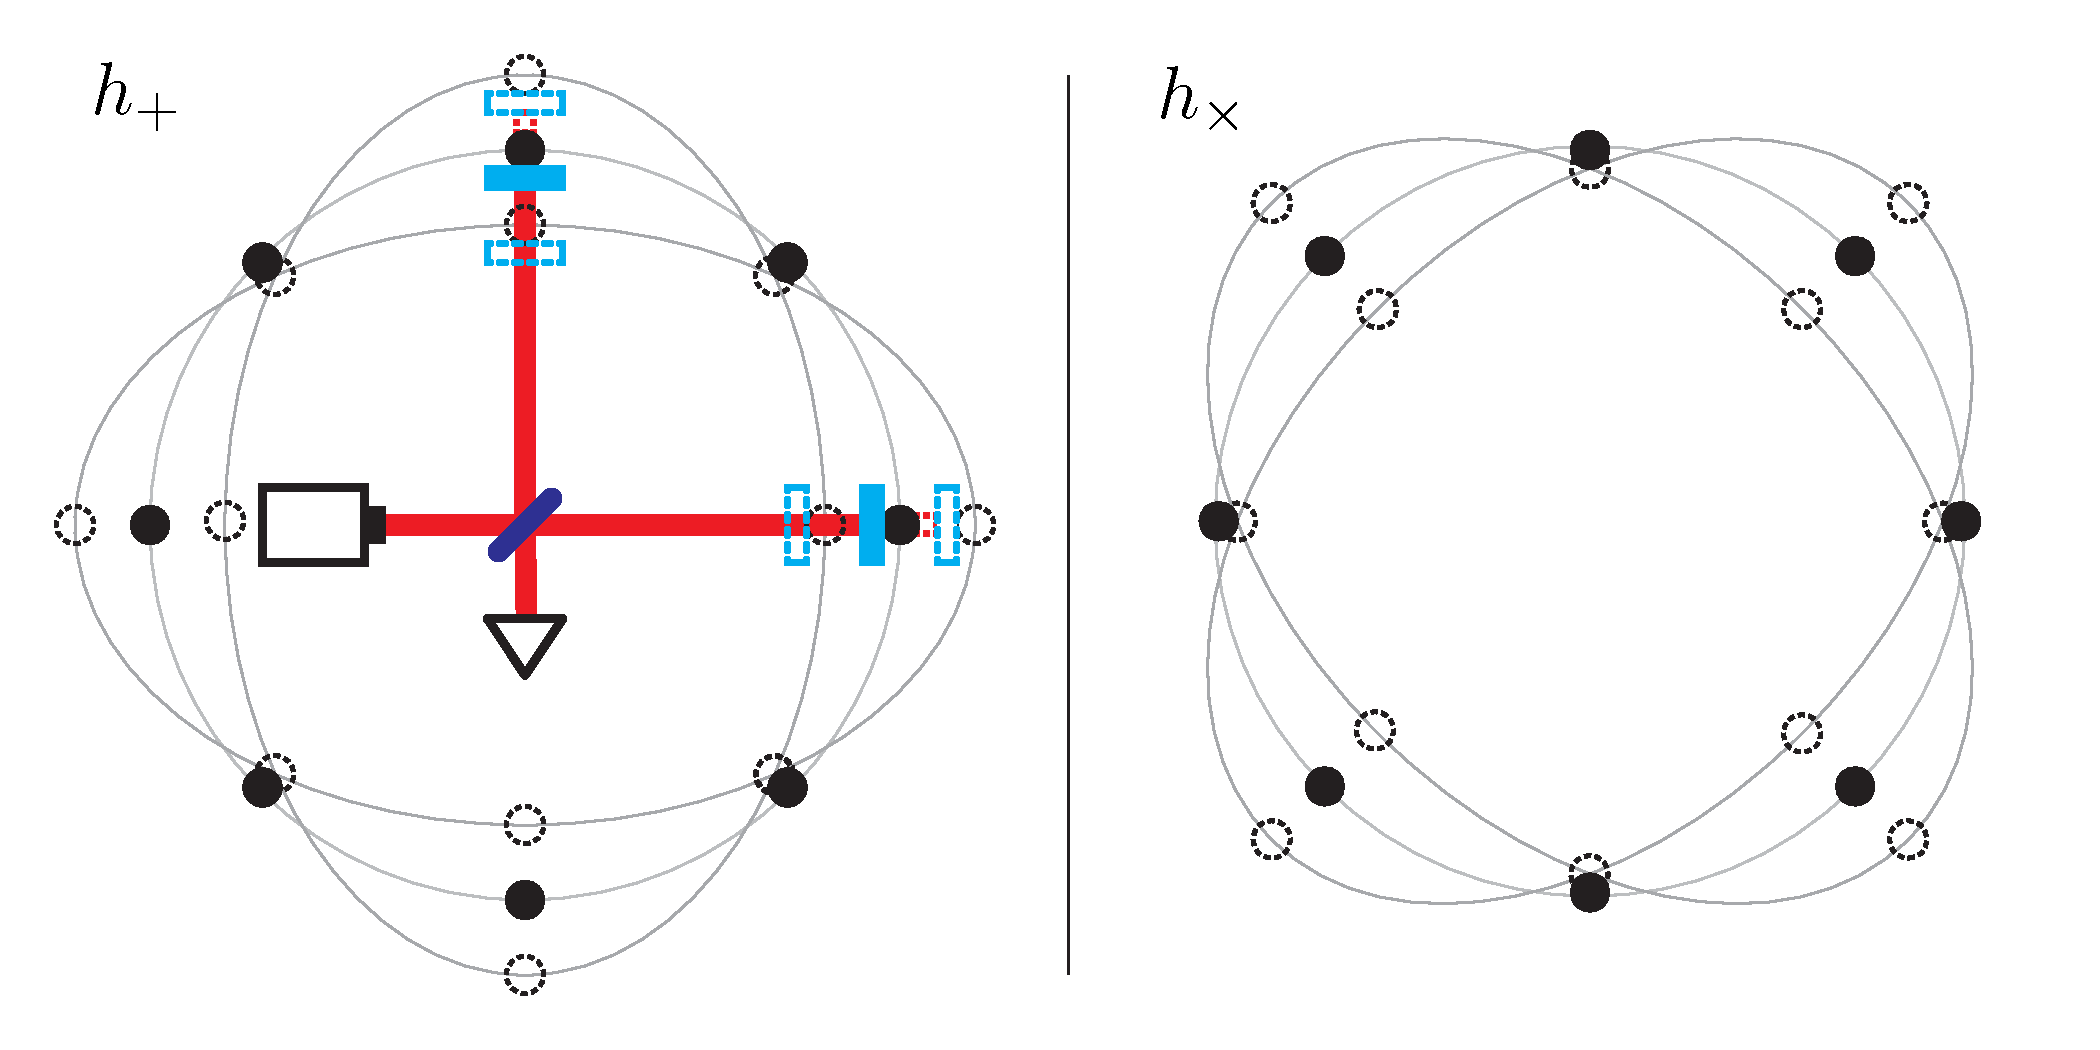
\includegraphics[width=6in]{figures/hpls-hcrs.pdf}
\caption{A diagram showing the effect of a passing gravitational wave on a ring of particles. The left diagram shows the effect of a $\pls$ polarized wave and the right shows the effect of $\crs$ polarized wave. On the $h_\pls$ diagram we have attached a mirror to the $+x$ and $+y$ particles. These form the end-test masses of the interferometer shown. For a discussion of how the interferometer works, see section \ref{sec:interferometry}.}
\label{fig:hpls-hcrs}
\end{figure}

\subsection{Gravitational Waves from a Compact Binary Inspiral}

We now consider the gravitational radiation emitted from a system consisting of two compact spherical objects orbiting around each other. Let the mass of the objects be denoted by $m_1$ and $m_2$, and the total mass by $M$. Consider their motion when they are at a distance $a \gg 2M$. We will assume their motion is determined entirely by their mutual gravitational attraction and that $m_1 \sim m_2 \sim \Msun$. Although we will find that the orbit of the objects shrinks due to the energy loss from emitted \acp{GW}, with these assumptions, $\dot{a} \ll v$, where $v$ is their relative orbital velocities. Thus we can assume quasi-stationary circular orbits. Additionally, since we have assumed $a \gg 2M$, $v \ll 1$; in this case, relativistic effects become negligible and we can use Newtonian gravity and Kepler's third law --- given by: 
\begin{equation}
\label{eqn:orbit_ang_v}
\Omega = \sqrt{\frac{M}{a^3}}
\end{equation}
where $\Omega$ is the orbital angular velocity --- to analyze the system.

Our assumptions also allow us to simplify equation \ref{eqn:wave_from_source}. First, from energy and momentum conservation ($T\indices{^{\mu\nu}_{,\nu}} = 0$) we have:
\begin{align*}
T\indices{^{00}_{,0}} &= -T\indices{^{0j}_{,j}} \\
T\indices{^{j0}_{,0}} &= -T\indices{^{jk}_{,k}}
\end{align*}
Doing some algebra yields:
\begin{equation*}
2T^{jk} = T\indices{^{00}_{,00}}x^jx^k - (T^{lm}x^jx^k)_{,ml} + 2(T^{lj}x^k + T^{lk}x^j)_{,l}
\end{equation*}
When we plug this into equation \ref{eqn:wave_from_source}\footnote{Since the background metric is $\eta_{\alpha\beta}$ we can lower the $ij$ indices on T with impunity.} we find that the last two terms are zero due to Stokes theorem. The $T^{00}$ term gives the mass-energy of the source, $\rho$. We therefore have:
\begin{equation}
\label{eqn:source_rho}
h^\TT_{ij} = 2 \left[ \partial_t^2 \int \frac{\rho(t - |\vec{x}-\vec{x}'|, \vec{x}')}{|\vec{x} - \vec{x}'|} \d^3x'\right]^\TT
\end{equation}

Now, because we are far from the source, $|\vec{x} - \vec{x}'| \sim r$ (where $r$ is the distance to the source), i.e., $|\vec{x}'|/|\vec{x}| \ll 1$. As is done in \ac{EM}, we can therefore expand the denominator \cite{ref:BlanfordThorne}:
\begin{equation}
\label{eqn:expansion}
\frac{1}{|\vec{x} - \vec{x}'|} = \frac{1}{r} + \frac{x^{j}x^{j'}}{r^3} + \frac{x^j x^k (3x^{j'}x^{k'} - r^{'2}\delta_{jk})}{2r^5} + \ldots
\end{equation}
Keeping the first term yields:
\begin{equation*}
\frac{2}{r} \partial_t^2 \int \rho(t - r) x^{'j}x^{'k} \d^3 x'
\end{equation*}
We recognize the integral as the second-time derivative of the second moment of the mass distribution, $\ddot{I}^{jk}$.\footnote{In general, we will use over-dots to indicate differentation with respect to proper time, $\tau$. However, because we are working in a Minkowski space time, $\tau \rightarrow t$. We can therefore use the dots here to indicate differentation with respect to the coordinate time.} Since we eventually remove the trace, we can instead use the mass quadrupole moment, $\qI_{jk}$, defined as:
\begin{equation}
\label{eqn:quad_moment}
\qI_{jk} = \int \rho(\mathbf{x})\left( x_j x_k - \frac{1}{3} \delta_{jk} \delta_{mn} x^{m} x^{n} \right) \d^3 x
\end{equation}
Plugging this into equation \ref{eqn:source_rho} yields:
\begin{equation}
\label{eqn:h_mass_quad}
h^{\TT}_{jk} = \frac{2}{r} \ddot{\qI}_{jk}^\TT(t - r)
\end{equation}
This is an important result: we only get gravitional waves if we have a changing quadrupole (or higher-order) moment. Contrast this with \ac{EM}, in which we only need a changing dipole moment to get electromagnetic waves.

Returning to our problem, to evaluate the amplitude of the \ac{GW} emitted by the binary we must first evaluate $\qI_{jk}$. Since we only have two masses, we can use the discreet form of the integral to directly write:
\begin{equation}
\label{eqn:discreet_qm}
\qI_{ij} = m_1(x_{1i}x_{1j} - \delta_{ij}\frac{1}{3} r_1^2) + m_2(x_{2i}x_{2j} - \delta_{ij}\frac{1}{3}r_2^2)
\end{equation}
where $r_n^2 = x_n^2 + y_n^2$ is the radial position of the $n\th$ mass. Working in the center-of-mass frame of the binary, we have:
\begin{align*}
x_1 &= r_1 \cos \Omega t \\
y_1 &= r_1 \sin \Omega t \\
x_2 &= - r_2 \cos \Omega t \\
y_2 &= - r_2 \sin \Omega t \\
\end{align*}
where
\begin{align}
r_1 &= a\frac{m_2}{m_1 + m_2} \\
r_2 &= a \frac{m_1}{m_1 + m_2}
\end{align}
Plugging these values into equation \ref{eqn:discreet_qm} we have:
\begin{align}
\qI_{xx} &= m_1 x_1^2 + m_2 x_2^2 - \frac{1}{3}(m_1r_1^2 + m_2r_2^2) \nonumber \\
         &= (m_1r_1^2 + m_2r_2^2)\left(\cos^2 \Omega t - \frac{1}{3}\right) \nonumber \\
         &= a^2\left(\frac{m_1m_2^2 + m_2m_1^2}{m_1+m_2}\right)\left(\cos^2 \Omega t - \frac{1}{3}\right) \nonumber \\
         &= \mu a^2 \left(\cos^2 \Omega t - \frac{1}{3} \right)
\end{align}
where:
\begin{equation}
\label{eqn:reduced_mass}
\mu = \frac{m_1 m_2}{M}
\end{equation}
is the reduced mass. By a similar calculation, we get:
\begin{align}
\qI_{yy} &= \mu a^2 \left(\sin^2 \Omega t - \frac{1}{3}\right) \\
         &= -\qI_{xx} \\
\qI_{zz} &= -\frac{1}{3} \mu a^2 \\
\qI_{xy} &= \mu a^2 \cos \Omega t \sin \Omega t \\
         &= \qI_{yx}
\end{align}
The second time derivative of the quadrupole moment is thus:
\begin{subequations}
\begin{align}
\ddot{\qI}_{xx} &=  -2\mu a^2\Omega^2 \cos(2\Omega t) \\
\ddot{\qI}_{yy} &=  2\mu a^2\Omega^2 \cos(2\Omega t)  \\
\ddot{\qI}_{xy} &=  -2 \mu a^2 \Omega^2 \sin(2 \Omega t) \\
                &=  \ddot{\qI}_{yx} \\
\ddot{\qI}_{zz} &=  0
\end{align}
\label{eqn:second_deriv_qm}
\end{subequations}

In order to plug equations \ref{eqn:second_deriv_qm} into equation \ref{eqn:h_mass_quad} we need the transverse part of the moments. We know that the gravitational waves will propagate outward from the binary. Therefore, if we project equations \ref{eqn:second_deriv_qm} into the spherical coordinates $\{r,\iota,\phi\}$ shown in figure \ref{fig:binary_coords}, then $\qI_{\iota\iota},~\qI_{\phi\phi},$ and $\qI_{\iota\phi}~ (= \qI_{\phi\iota})$ will form the parts of the tensor transverse to the propagation. Since the $z$ components of the time derivative of the quadrupole are all zero, the transformation law is simplified to:
\begin{align*}
\ddot{\qI}_{i'j'}  &= \Lambda\indices{_{i'}^i} \Lambda\indices{_{j'}^j} \ddot{\qI}_{ij} \\
            &= \Lambda\indices{_{i'}^x} \Lambda\indices{_{j'}^x} \ddot{\qI}_{xx} + \Lambda\indices{_{i'}^x} \Lambda\indices{_{j'}^y} \ddot{\qI}_{xy} + \Lambda\indices{_{i'}^y} \Lambda\indices{_{j'}^x} \ddot{\qI}_{yx} + \Lambda\indices{_{i'}^y} \Lambda\indices{_{j'}^y} \ddot{\qI}_{yy}
\end{align*}
We can further simplify the problem by setting the initial orbital phase, $\phi$, to 0. Since we have assumed quasi-stationary circular orbits, we can later account for arbitrary initial phase by letting $\Omega t \rightarrow \Omega t + \phi$. Doing so simplifies the transformation matrix to:
\begin{equation*}
\Lambda = \begin{pmatrix}
    \sin \iota &    0    &  \cos \iota \\
    \cos \iota &    0    &  -\sin \iota \\
         0     &    1    &    0
    \end{pmatrix}
\end{equation*}
Resulting in:
\begin{align*}
\ddot{\qI}_{\iota\iota} &= \ddot{\qI}_{xx} \cos^2\iota \\
\ddot{\qI}_{\phi\phi}   &= \ddot{\qI}_{yy} \\
\ddot{\qI}_{\iota\phi}  &= \ddot{\qI}_{xy} \cos \iota \\
                        &= \ddot{\qI}_{\phi\iota}
\end{align*}
To make the tensor traceless in this coordinate basis, we set $\ddot{\qI}^{\TT}_{\iota\iota} = -\ddot{\qI}^{\TT}_{\phi\phi} = 1/2(\ddot{\qI}_{\iota\iota} - \ddot{\qI}_{\phi\phi})$. Letting $\Omega t \rightarrow \Omega t - \phi$, we have:
\begin{align}
\ddot{\qI}^{\TT}_{\iota\iota} &= \mu a^2 \Omega^2 \cos(2[\Omega t - \phi])(1 + \cos^2\iota) \\
\ddot{\qI}^{\TT}_{\iota\phi}  &= -2 \mu a^2 \Omega^2 \sin(2[\Omega t - \phi])\cos\iota
\end{align}
Plugging this into equation \ref{eqn:h_mass_quad}, and using Kepler's law to put $a$ in terms of $M$ and $\Omega$ ($a = \left(M/\Omega^2\right)^{1/3}$), we have:
\begin{subequations}
\label{eqn:h_pls-h_crs}
\begin{align}
h^{\TT}_{\iota\iota} &= \frac{2}{r}\mu (M \Omega)^{2/3} \cos(2[\Omega (t-r) - \phi])(1 + \cos^2\iota) &= h_{\pls} \\
h^{\TT}_{\iota\phi}  &= -\frac{4}{r} \mu (M\Omega)^{2/3} \sin(2[\Omega (t-r) - \phi])\cos\iota &= h_{\crs}
\end{align}
\end{subequations}
Here we have identified the $\iota\iota$ and $\iota\phi$ parts of the \ac{GW} field as the ``plus" and ``cross" polarizations by using the basis vectors \cite{ref:BlanfordThorne}:
\begin{equation}
\mathbf{e}^{\pls} = (\vec{e}_{\iota} \otimes \vec{e}_{\iota} - \vec{e}_{\phi} \otimes \vec{e}_{\phi}), ~ \mathbf{e}^{\crs} = (\vec{e}_{\iota} \otimes \vec{e}_{\phi} + \vec{e}_{\phi} \otimes \vec{e}_{\iota})
\end{equation}
In equations \ref{eqn:h_pls-h_crs} we can see that the gravitational-wave frequency is \emph{twice} the orbital frequency:
\begin{equation}
\label{eqn:f_GW}
\fGW = 2 f_{\mathrm{orbit}} = \frac{\Omega}{\pi}
\end{equation}

The inclination angle, $\iota$, and the distance to the center of mass, $r$, are \emph{extrinsic} parameters of the binary: they depends only on the orientation of the binary with respect to an outside observer. To separate the part of the waveform that depends on the \emph{intrinsic} parameters of the binary --- i.e., the physical parameters of the binary that are independent of the location of the observer\footnote{When we say ``independent of the location of the observer" we actually mean ``independent of the location of any observers that are in the same \ac{LLF}."} --- we define the \emph{sine chirp}, $h_s$, and the \emph{cosine chirp}, $h_c$ \cite{ref:Brown}:
\begin{subequations}
\label{eqn:cos_sin_chirp}
\begin{align}
h_c &\equiv 2 \mu (M \Omega^{2/3}) \cos(2[\Omega t - \phi_0] ) \\
h_s &\equiv 2 \mu (M \Omega^{2/3}) \sin(2[\Omega t - \phi_0] )
\end{align}
\end{subequations}
such that:
\begin{subequations}
\label{eqn:hpls_hcrs}
\begin{align}
h_\pls &= \frac{h_c}{r} (1 + \cos^2\iota) \\
h_\crs &= \frac{h_s}{r} \cos\iota
\end{align}
\end{subequations}
(The reason for the name ``chirp" will become clear below.) Here, $\phi_0$ is the phase of the binary at some initial point in time.

\begin{figure}
\center
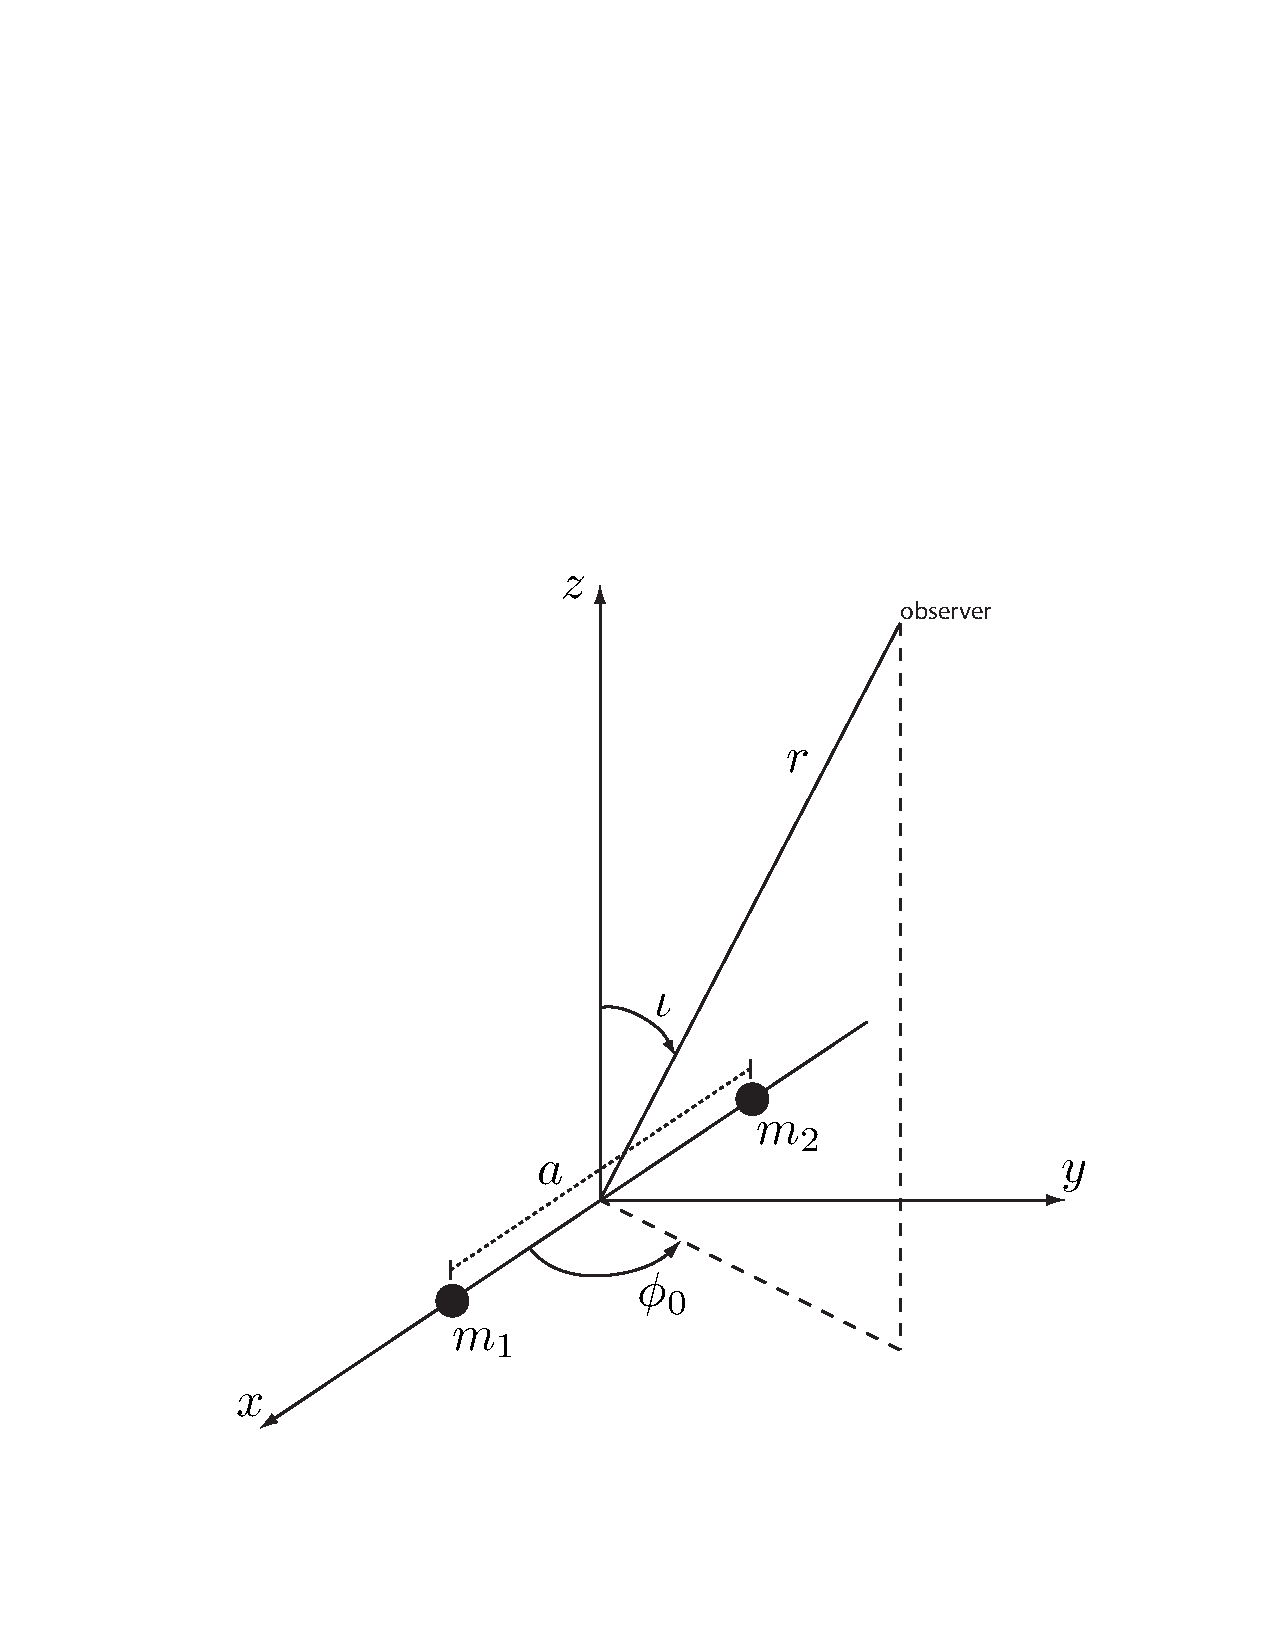
\includegraphics[height=5in]{figures/binary.pdf}
\caption{The center-of-mass frame of a binary with separation distance $a$. The coordinates $\{r,\iota,\phi\}$ give, respectively, the distance to an observer, the inclination angle of the observer, and the phase of the binary. $\phi_0$ is the initial phase. Figure originally published in \cite{ref:Brown}.}
\label{fig:binary_coords}
\end{figure}


\subsection{Evolution of the Gravitational Waveform in Newtonian Physics}
\label{sec:0pn_solution}

In Chapter \ref{ch:pipeline_principles} we will find that we use the sine and cosine waveforms to \emph{match-filter} data from \ac{GW} detectors. Match filtering offers the best way to find a \ac{CBC} \ac{GW} signal that is buried in noise. However, to perform the match filter, we need to generate a time or frequency series for the waveform. From equations \ref{eqn:cos_sin_chirp} we see that this requires knowledge of how the orbital phase, $\Omega t$, (or, via equation \ref{eqn:f_GW}, the gravitational-wave phase) evolves with time (or frequency). We can find this by considering the energy lost by the binary due to gravitational radiation.

Using equation \ref{eqn:h_mass_quad} it can be shown that the energy loss from \ac{GW} emmision is given by \cite{ref:BlanfordThorne}:
\begin{equation}
\label{eqn:energy_loss-t}
\frac{\d E}{\d t} = -\frac{1}{5}\left< \dddot{\qI}_{jk} \dddot{\qI}^{jk} \right>
\end{equation}
where the brackets $<\cdot>$ denote an average over time. Using equations \ref{eqn:second_deriv_qm}, we find:
\begin{align*}
\dddot{\qI}_{xx} &= 4 \mu a \Omega^3\sin(2\Omega t) = -\dddot{\qI}_{yy} \\
\dddot{\qI}_{xy} &= -4 \mu a^2 \Omega^3\cos(2\Omega t) = \dddot{\qI}_{yx}
\end{align*}
This gives:
\begin{align*}
\frac{\d E}{\d t} &= -\frac{2}{5}\left< \ddot{\qI}_{xx}^2 + \ddot{\qI}_{xy}^2 \right> \\
    &= -\frac{32}{5} \mu^2 a^4 \Omega^6 \left< \sin^2(2\Omega t) + \cos^2(2\Omega t) \right> \\
    &= -\frac{32}{5} \frac{\mu^2 M^3}{a^5}
\end{align*}
In the last step we have again used Kepler's law to put $\Omega$ in terms of $M$ and $a$. We can use this equation to find how the separation distance shrinks with time. Using the chain rule we have:
\begin{equation}
\label{eqn:energy_loss-a}
\frac{\d E}{\d t} = \frac{\partial E}{\partial a}\frac{\d a}{\d t}
\end{equation}
From Newton's law of gravity and conservation of energy, the binary's energy is related to the separation distance by:
\begin{equation*}
\frac{\partial E}{\partial a} = \frac{\mu M}{2a^2}
\end{equation*}
Plugging this into equation \ref{eqn:energy_loss-a} yields:
\begin{equation*}
\frac{1}{2} a^3 \d a = -\frac{32}{5} \mu M^2 \d t
\end{equation*}
Integrating this from some initial separation, $a_0$, at time $t_0$, to the separation, $a$, at some arbitrary time $t$ gives:
\begin{equation}
\label{eqn:a_evolution}
a = a_0 \left(1 - \frac{t-t_0}{\tau_0} \right)^{1/4}
\end{equation}
where:
\begin{equation}
\label{eqn:tau_0-a}
\tau_0 = \frac{5}{256} \frac{a_0^4}{\mu M^2}
\end{equation}
is the \emph{time to coalescence}. That is, $\tau_0$ is the amount of time it takes for the binary to go from the initial separation $a_0$ to $a=0$. In equation \ref{eqn:a_evolution} we can see that the orbital separation decreases with time due to the loss in energy. In other words, the two masses ``inspiral" into each other.

We can use equations \ref{eqn:a_evolution} and \ref{eqn:tau_0-a}, and Kepler's third law to find how the orbital angular velocity changes with time. Re-arranging equation \ref{eqn:keplers_thirdlaw} to $a = (M/\Omega^2)^{1/3}$ and manipulating equation \ref{eqn:tau_0-a} to get $a_0$ in terms of $\tau_0$, we have, from equation \ref{eqn:a_evolution}:
\begin{equation*}
M^{4/3}\Omega^{-8/3} = \frac{256}{5} \mu M^2(\tau_0 - t)
\end{equation*}
Here, we have set the initial time $t_0 = 0$. Rearranging, we have:
\begin{equation}
\label{eqn:omega_evolution}
\Omega = \left[ \frac{5}{256} \frac{1}{\eta M^{5/3}(\tau_0 - t)} \right]^{3/8}
\end{equation}
where:
\begin{equation}
\label{eqn:symmetric_mass}
\eta \equiv \frac{\mu}{M}
\end{equation}
is the \emph{symmetric mass-ratio}. Using equation \ref{eqn:f_GW} to relate the gravitational-wave frequency to $\Omega$, we find:
\begin{equation}
\label{eqn:f_evolution}
\fGW(t) \propto (\tau_0 - t)^{-3/8}
\end{equation}
Figure \ref{fig:GW_evolution-freq} shows what the gravitational-wave frequency looks like as a function of time. We see that the wave sweeps upward in frequency in a ``chirp" pattern, asymptoting to infinity as $a \rightarrow 0$.

We can also use equation \ref{eqn:omega_evolution} to find how the amplitude of the waveform changes over time. In equations \ref{eqn:cos_sin_chirp} we see that the amplitude of the waveform is proportional to $M\Omega^{2/3}$. Thus:
\begin{equation}
\label{eqn:amp_evolution}
|h_c| = |h_s| = 2 \left( \frac{5}{256} \frac{\mchirp}{\tau_0 - t} \right)^{1/4}
\end{equation}
where we have defined the \emph{chirp mass}, $\mchirp$, as:
\begin{equation}
\mchirp \equiv \eta^{3/5}M
\end{equation}
Thus the amplitude also increases with time, asymptoting to infinity as $a \rightarrow 0$. Figure \ref{fig:GW_evolution-waveform} shows what the waveform evolution looks like for an equal mass binary ($\eta=1/4)$).

\begin{figure}[htbp]
\center
\subfigure[$f(t)$]{\label{fig:GW_evolution-freq}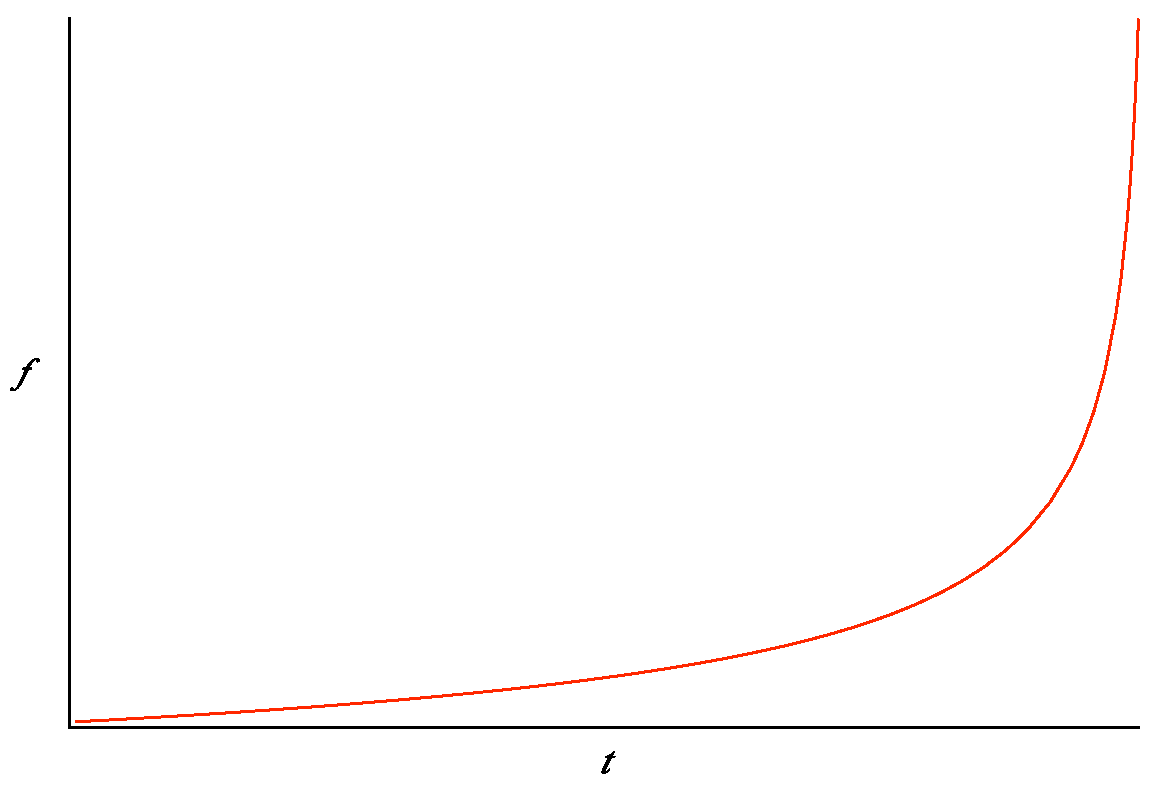
\includegraphics[height=3in]{figures/foft_plot.pdf}}
\subfigure[$h(t)$]{\label{fig:GW_evolution-waveform}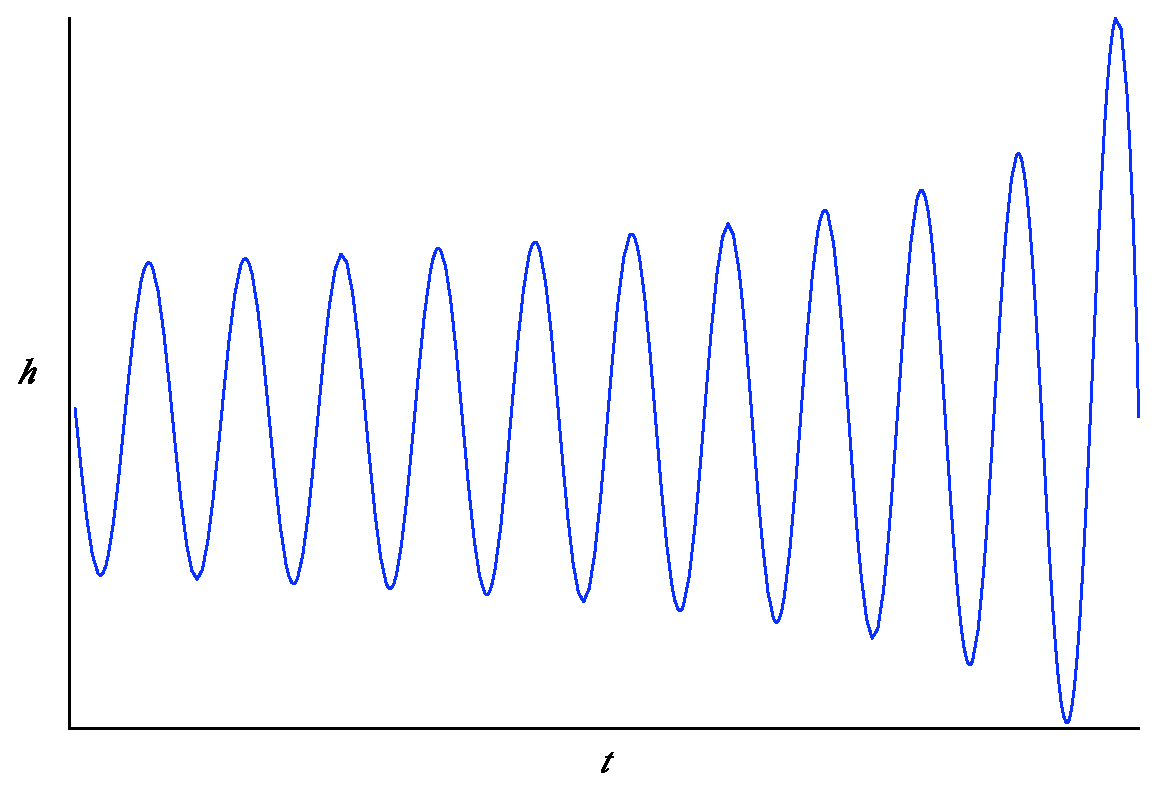
\includegraphics[height=3in]{figures/hoft_plot.pdf}}
\caption{The frequency evolution and waveform evolution of an equal mass binary using equations \ref{eqn:f_evolution} and \ref{eqn:amp_evolution}. Frequency, amplitude, and time are given in arbitrary values; the time in the two plots is not to scale.}
\label{fig:GW_evolution}
\end{figure}


\subsection{Orbital Dynamics in a Schwarzschild Spacetime}
\label{sec:schwarzchild_dynamics}

In the above analysis we assumed the relative velocities of the binary's component masses were small compared to the speed of light, and that the spacetime curvature was relatively flat. This allowed us to use Newtonian and Keplerian dynamics to analyze the binary. While this worked well when the masses were far apart from each other, it breaks down as the separation distance gets small. This was evident in the fact that the orbital angular velocity asymptoted to infinity as $a \rightarrow 0$. This means that the component masses' relative tangential velocity:
\begin{equation}
v = (M\Omega)^{1/3}
\end{equation}
would also approach infinity. Clearly there is a separation distance for which our assumptions fail, and we must take into account relativistic effects.

To illustrate relativistic effects, we consider a test-particle with mass $m$ orbiting a massive black hole with mass $M$, such that $m \ll M$. For simplicity we will assume that both the test mass and the black hole have negligible spin. Thus, we can describe the spacetime using the Schwarzchild metric \cite{ref:MTW}:
\begin{equation}
\d s^2 = - (1 - 2M/r)\d t^2 + \frac{\d r^2}{1 - 2M/r} + r^2\d\phi^2 + r\sin\iota \d\iota^2
\end{equation}
The coordinates are chosen such that $r=0$ is at the center-of-mass of the system, which --- since $M \gg m$ --- is roughly at the ``center" of the black hole. Without loss in generality we will assume the inclination angle is equal to $\pi/2$, so that the $\d\iota$ part of the line element is $0$.\footnote{For a treatment of this problem with $\iota \neq \pi/2$ see Box 25.4 of \cite{ref:MTW}.} In this case the metric only has three elements:
\begin{subequations}
\begin{align}
g_{tt} &= - (1 - 2M/r) \\
g_{rr} &= (1-2M/r)^{-1} \\
g_{\phi\phi} &= r^2
\end{align}
\end{subequations}

In the last section the equation of motion for the masses was given by Kepler's third law, which related the orbital angular velocity to the mass and separation distance. To analyze the test particle's orbital evolution we again need an equation of motion. However, since we are working in a curved spacetime it is not clear that Kepler's third law still holds. To find the relativistic equation of motion, we consider the particle's geodesic path as it orbits the black hole. Since no external forces act on the particle, the geodesic equation is \cite{ref:MTW, ref:Schutz, ref:Carroll}:
\begin{equation}
\frac{\d^2 x^{\alpha}}{\d \tau^2} + \Gamma\indices{^\alpha_{\mu \nu}} \frac{\d x^{\mu}}{\d\tau} \frac{\d x^{\nu}}{\d\tau} = 0
\end{equation}
where the Christoffel symbol is:
\begin{align}
\label{eqn:christoffel_symbols}
\Gamma\indices{^\alpha_{\mu\nu}} &= g^{\alpha\sigma}\Gamma\indices{_{\sigma\mu\nu}} \nonumber \\
    &= \frac{1}{2}g^{\alpha\sigma}( g_{\sigma\mu,\nu} + g_{\sigma\nu,\mu} - g_{\mu\nu,\sigma}) \nonumber \\
    &= \frac{1}{2}g^{\alpha\alpha}(g_{\alpha\mu,\nu} + g_{\alpha\nu,\mu} - g_{\mu\nu,\alpha})
\end{align}
In the last step we have used the fact that there are no mixing terms in the metric (i.e., $g^{\alpha\sigma} = \delta\indices{^{\alpha}_\sigma}g^{\alpha\sigma}$). 

Before analyzing these equations, we note a few properties of the metric which greatly simplify the problem. The metric has no $t$, $\phi$, or (since we set the particle's inclination angle to $\pi/2$) $\iota$ dependence. Thus the $t$, $\phi$, and $\iota$ components of the particle's conjugate four-momentum, $p_\alpha$ are conserved \cite{ref:MTW, ref:Schutz, ref:Carroll}. The particle's four-momentum is given by:
\begin{equation}
p^{\alpha} = m u^{\alpha} = m \frac{\d x^\alpha}{\d\tau}
\end{equation}
where $u^{\alpha}$ is the particle's four-velocity. The four-momentum is related to the conjugate momentum by: $p^{\alpha} = g^{\alpha\beta}p_{\alpha}$. Since $p_{\alpha}$ has no $\tau$ dependence, and since $g^{\alpha\beta}$ only depends on $r$, $\dot{p}^{\alpha} \sim \dot{r}$. (Dots over the coordinates indicate differentation with respect to the proper time.) We shall assume, as we did in the previous section, that $\dot{r} \ll \dot{\phi}$, i.e., that the particle follows quasi-stationary orbits. In this case, $\dot{r} \approx 0$, as well as $\ddot{r}$. Thus: 
\begin{equation}
\dot{p}^t = \ddot{t}/m = \dot{p}^\phi = \ddot{\phi}/m = \dot{p}^\iota = \ddot{\iota}/m = 0
\end{equation}
Since we have fixed the inclination angle to $\pi/2$, $\ddot{\iota}$ is also zero. From equation \ref{eqn:christoffel_symbols}, this means that $\Gamma\indices{^\iota_{\mu\nu}}$ is zero, and so the $\iota$ equation of motion gives the trival result $0 = 0$. Thus we only have three equations to consider:
\begin{equation}
\label{eqn:equations_of_motion}
\Gamma\indices{^\alpha_{tt}} \dot{t}^2 + 2\Gamma\indices{^\alpha_{t\phi}}\dot{t}\dot{\phi} + \Gamma\indices{^\alpha_{\phi\phi}} \dot{\phi}^2 = 0 
\end{equation}
where $\alpha = r,t,\phi$. We further simplify these equations by noting:
\begin{align*}
\Gamma\indices{^\alpha_{tt}} &= \frac{1}{2} g^{\alpha\alpha}(2g_{\alpha t,t} - g_{tt,\alpha}) &= -\frac{1}{2} g^{\alpha\alpha}g_{tt,\alpha} \\
\Gamma\indices{^\alpha_{\phi\phi}} &= \frac{1}{2} g^{\alpha\alpha}(2g_{\alpha \phi,\phi} - g_{\phi\phi,\alpha}) &= -\frac{1}{2} g^{\alpha\alpha}g_{\phi\phi,\alpha} \\
\Gamma\indices{^\alpha_{t\phi}} &= \frac{1}{2} g^{\alpha\alpha}(g_{\alpha t,\phi} + g_{\alpha \phi,t} - g_{t\phi,\alpha}) &= 0 \\
\end{align*}
Since $g_{tt,\alpha}$ and $g_{\phi\phi,\alpha}$ are only non-zero if $\alpha = r$, the only non-zero Christoffel symbols are $\Gamma\indices{^r_{tt}}$ and $\Gamma\indices{^r_{\phi\phi}}$. This means the only non-trival equation of motion is the one for which $\alpha = r$. The non-zero Christoffel symbols are:
\begin{subequations}
\begin{align}
\Gamma\indices{^r_{tt}} &= -\frac{1}{2} g^{rr}g_{tt,r} &= \frac{M}{r^2}(1 - 2M/r) \\
\Gamma\indices{^r_{\phi\phi}} &= -\frac{1}{2} g^{rr}g_{\phi\phi,r} &= -r(1-2M/r)
\end{align}
\end{subequations}
Plugging these into the equation of motion yields:
\begin{align*}
\frac{M}{r^2}(1 - 2M/r)\dot{t}^2 - r(1-2M/r)\dot{\phi}^2 = 0 \\
\Rightarrow \frac{\dot{\phi}^2}{\dot{t}^2} = \frac{M}{r^3}
\end{align*}
Note that:
\begin{equation}
\frac{\dot{\phi}}{\dot{t}} = \frac{\d\phi/\d\tau}{\d t/\d\tau} = \frac{\d\phi}{\d t} = \Omega
\end{equation}
where $\Omega$ is the angular velocity of the test particle as measured by an observer in the particle's \ac{LLF}. Thus we have:
\begin{equation}
\Omega = \sqrt{\frac{M}{r^3}}
\end{equation}
Evidently Kepler's third law is valid for all $r$; i.e., it is a relativistic equation. 

As noted above, $\dot{\phi} = p^\phi/m$ and $\dot{t} = p^t/m$. We can therefore write:
\begin{equation}
\label{eqn:eom1}
\frac{p^\phi}{p^t} = \sqrt{\frac{M}{r^3}}
\end{equation}
Now, since $p_t$ and $p_\phi$ are conserved, we can set them equal to the constants $-E$ and $L$, respectively. We can identify these constants as the particle's energy and momentum as seen by an observer at $r = \infty$ \cite{ref:Schutz}. Raising the indices, we have:
\begin{align}
p^t &= g^{tt}p_t &= \frac{E}{1-2M/r} \\
p^\phi &= g^{\phi\phi}p_\phi &= \frac{L}{r^2}
\end{align}
The equation of motion \ref{eqn:eom} is therefore:
\begin{equation}
\label{eqn:eom2}
\frac{(1-2M/r)L}{r^2E} = \sqrt{\frac{M}{r^3}}
\end{equation}
We can put $L$ in terms of $E$ by noting:
\begin{equation*}
p^{\alpha}p^{\beta}g_{\alpha\beta} = p^{\alpha}p_{\alpha} = m^2 u^{\alpha}u_{\alpha} = -m^2
\end{equation*}
Since $p^r$ and $p^\iota$ are both zero,
\begin{equation*}
p^{\alpha}p_{\alpha} = p^t p_t + p^\phi p_\phi = -\frac{E^2}{1-2M/r} + \frac{L^2}{r^2} = -m^2
\end{equation*}
Rearranging this gives:
\begin{equation}
L = r\sqrt{\frac{E^2}{1-2M/r} - m^2}
\end{equation}
Plugging this into equation \ref{eqn:eom2} yields:
\begin{equation}
\label{eqn:Eschwarz}
E = m\frac{1-2M/r}{\sqrt{1-3M/r}}
\end{equation}
We have arrived at a solution for the particle's energy as a function of its oribital distance. (Note that as $r\rightarrow \infty$, $E \rightarrow m$, meaning $E$ becomes the rest-mass energy of the particle, as expected.) 

Figure \ref{fig:Eofr} shows a plot of $E/m$ as a function of $r/M$. From this (or by taking the derivative of equation \ref{eqn:Eschwarz} and setting it equal to zero) we can see that $E/m$ decreases monontonically from inifinity, until it reaches a minimum at $r=6M$. Keep in mind that we obtained this graph by considering quasi-stationary circular orbits. Thus the plot shows how much energy is needed at each $r$ for the particle to maintain a circular orbit. This means that at radii $\geq 6M$ the particle can sustain stable circular orbits without needing any additional energy. Below $r=6M$, however, energy must be added to the particle in order for it to sustain its orbit.\footnote{And below $r=2M$ an infinite amount of energy would be needed for the particle to sustain a stable orbit. Thus $r=2M$ is the event horizon of the black hole, also known as the Schwarschild radius.} Assuming the system evolves adiabatically (that is, no external energy is added), after the particle passes $r=6M$ it will cease to inspiral and will plunge into the black hole. This part of the evolution is known as ``merger."

The point $r=6M$ is known as \ac{ISCO}. At this point our analysis, both in this section and the last, breaks down since we can no longer assume $\dot{r} \ll \dot{\phi}$. The phase and amplitude evolution of the gravitational wave emitted after this point must therefore be evaluated using more sophisticated techniques. Although we found this radius by considering a Schwarschild metric, an \ac{ISCO} will exist for equal-mass systems as well (it may not occur at $r=6M$, however).

The systems we will consider in this thesis have masses low enough that the frequencies of their emitted \acp{GW} are of order a few kHz when they pass \ac{ISCO}. Since our gravitational-wave detectors have low sensitivity at these frequencies (see section \ref{sec:interferometers}) we can simply terminate the matched filter at $f_{\mathrm{isco}}$, which is the frequency of the gravitational wave when the source's component masses pass \ac{ISCO}. This permits us to use the techniques outlined in the last section and the next to generate a \ac{GW} waveform.

\begin{figure}[tbp]
\center
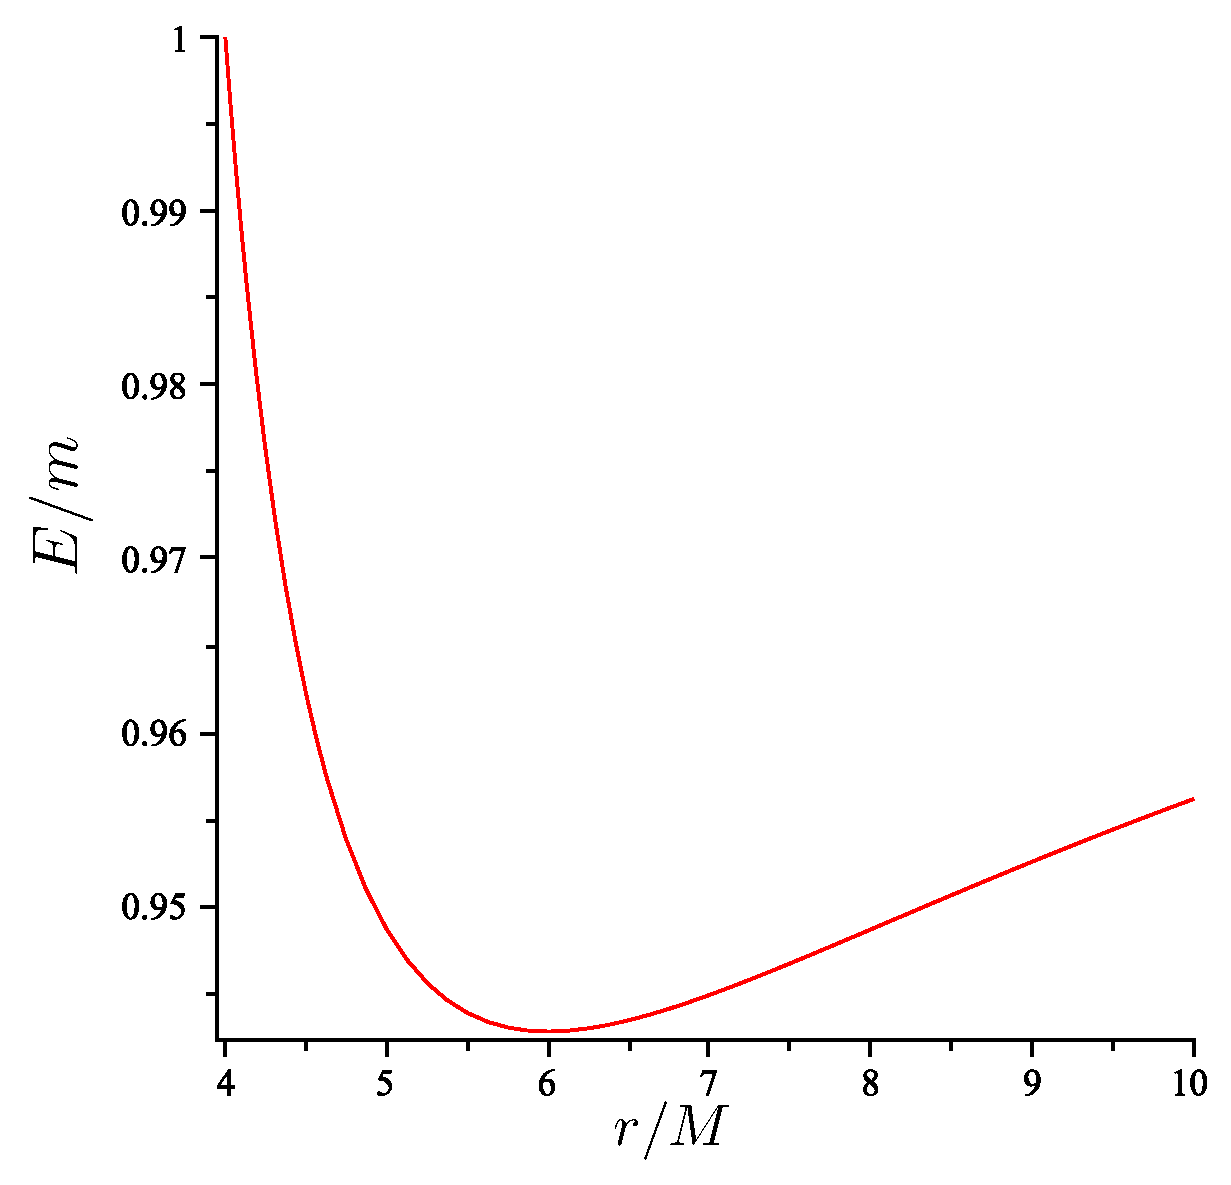
\includegraphics[width=4in]{figures/Eofrplot.pdf}
\caption{A plot of the energy-per-unit mass of a test particle orbiting a Schwarschild black hole as a function of its radial coordinate per the black hole's mass. The plot was created in Maple using equation \ref{eqn:Eschwarz}.}
\label{fig:Eofr}
\end{figure}

\subsection{The Post-Newtonian Approximation}

Let us recap the steps we took in section \ref{sec:0pn_solution} to arrive at a solution for the gravitational waveform:
\begin{itemize}
\item{First, we performed a multipolar expansion on the right hand side of equation \ref{eqn:} to get $h^\TT_{ij}$ in terms of increasing moments of the mass-energy density. This eventually allowed us to solve the \emph{energy-balance equation}:
\begin{equation}
\label{eqn:energy_balance}
\frac{\d E}{\d t} = -\mathcal{F}
\end{equation}
Since we only kept the first (most-dominant) term of the expansion, we had $\mathcal{F} = \left<\dddot{\qI_{jk}}\dddot{\qI^{jk}}\right>/5$.}
\item{Next, we found an expression for $E$ in terms of the mass and the orbital sepration. In section \ref{sec:0pn_solution} we used using Newton's law of gravity to find $E$. In section \ref{sec:schwarz_dynamics} we were a bit more sophisticated, and we obtained $E$ by using the Schwarzschild metric.}
\item{Plugging our expression for $E$ into the energy balance equation, we were able to find how the phase and amplitude of the \ac{GW} evolved with time.}
\end{itemize}
Generalizing, this process is known as the \emph{post-Newtonian approximation}.

If our fortitude and skill permitted, we could have kept higher order terms in the mutipolar expansion of $h$, which would have given us a more complicated experssion for $\mathcal{F}$. However, had we limited ourselves to the mass-moments, we would have missed some important terms. If we perform the multipolar expansion and take the integral \emph{before} taking the transverse-traceless part, we would have found that the $h_{0j}$ terms yield corrections to the gravitational wave from moments of the momentum density. In general, we would get \cite{ref:BlanfordThorne}:
\begin{equation}
|h_\pls| \sim |h_\crs| \sim \frac{\ddot{\qI_2}}{r} \& \frac{\dddot{\qI_3}}{r} \& \ldots \& \frac{\ddot{\mathcal{S}}}{r} \& \frac{\dddot{\mathcal{S}}}{r} \& \ldots
\end{equation}
Here, $\&$ indicates addition with terms, and:
\begin{equation}
\qI_l \sim ML^l, \quad \mathcal{S}_l \sim MvL^l
\end{equation}
are the mass and momentum moments, respectively, of order $l$. $L$ is the size of the source and $v$ is the relative velocities of the objects. Since the number of time derivatives grows with each of these terms, we can see that each term grows as $\partial_t^{(2-l)} L \sim v^{(2-l)}$. Hence the effects from each term becomes more relevant as the relative velocity of the objects grows.\footnote{Since $\mathcal{S} \sim Mv$, its effect on $h$ is one-step down from the mass-moment. In other words, $|\mathcal{S}_l| \sim |\qI_{l-1}|$. For example, the mass quadrupole ($l=2$) goes as $v^0$, where as the momentum quadrupole goes as $v^1$. Due to conservation of angular momentum, the $\mathcal{S}_1$ term, like the $\qI_1$ term, has no effect on $h$. Thus the dominant term is the mass-quadrupole ($\qI_2$), and so we were ok neglecting the momentum moments in section \ref{sec:first_approx}.}

To find the an expression for $E$ in section \ref{sec:first_approx} we used Newtonian physics. If we consider relativistic effects due to spacetime curvature, as we did in section \ref{sec:schwarzchild_dynamics}, we find that we can also express $E$ in terms of a power series in $v$. For example, in the Schwarzschild case above, we can re-work equation \ref{eqn:} by noting that $v = r\Omega$. Using equation \ref{eqn:} we get:
\begin{equation}
v = \sqrt{\frac{M}{r}}
\end{equation}
Thus we can re-write equation \ref{eqn:} as:
\begin{equation}
E = m \frac{1-2v^2}{\sqrt{1-3v^2}}
\end{equation}
Since $v \ll 1$, we can write expand the denominator in a Maclaurin series, which results in:
\begin{equation}
\frac{E}{m} = 1 - \frac{1}{2}v^2 + \frac{3}{8}v^4 + \mathcal{O}(v^6)
\end{equation}
To relate this to the phase of the gravitational wave, $\phi$, we use the chain rule to write:
\begin{equation}
\frac{\d E}{\d t} = \frac{\d E}{\d v}\frac{\d v}{\d \phi}\frac{\d \phi}{\d t}
\end{equation}
We can get $\d \phi / \d t$ by noting that:
\begin{equation}
\phi = \int 2\pi \fGW \d t
\end{equation}
thus:
\begin{equation}
\frac{\d \phi}{\d t} = 2\pi \fGW
\end{equation}
Also note that, from equation \ref{eqn:},
\begin{equation}
\label{eqn:v_to_f}
v = (\pi m \fGW)^{1/3}
\end{equation}
We can therefore write:
\begin{equation}
\frac{\d \phi}{\d t} = \frac{2 v^3}{m}
\end{equation}
Plugging these results into the energy balance equation, rearranging terms, and integrating yields:
\begin{equation}
\phi(v) = \phi_0 + 2\int_{v}^{v_0} \frac{v^3 (\d E/\d v)}{\mathcal{F}(v)} \d v
\end{equation}
Here, $\phi_0$ is the \ac{GW} phase of the binary at the initial velocity $v_0$. (If we instead prefer $\phi$ as a function of $\fGW$ we can use equation \ref{eqn:v_to_f} to convert.) Thus, by expanding $\mathcal{F}$ and $E$ to some desired power of $v$, and performing the integral, we can obtain higher order corrections to the gravitational wave.

How \ac{pN} expansions are carried out to various orders is a rich (and complicated) field that is beyond the scope of this thesis. Here, we only note a few properties that are relevant to the low-mass \ac{CBC} search that we will describe in later chapters:
\begin{itemize}
\item{Each successive term in the expansion of $\mathcal{F}$ accounts for additional physics of the binary. For example, the ``0\ac{pN}" order ($\sim v^0$) results in \acp{GW} from a changing mass-quadrupole. We were able to compute the effects of this order above, in section \ref{sec:}. The ``1\ac{pN}" order ($\sim v^2$), which takes into account the mass-octopole and momentum-quadrupole, results in the perihelion shift of orbiting bodies. The next step is the ``1.5\ac{pN}" term\footnote{The numbering of the \ac{pN} orders increase by $0.5$ because they are based on powers of $M/r$.} ($\sim v^3$), which results in frame dragging. Thus it takes into account the effects of spin/orbit coupling. It also adds a correction for outgoing waves that scatter off of the binary's spacetime curvature, known as the ``wave-tail". At 2\ac{pN} we get effects from spin/spin coupling; at 2.5\ac{pN} order we get effects from ``radiation-reaction"; etc.}
\item{As described in the next chapter, in the low-mass \ac{CBC} search we look for \acp{GW} by match filtering gravitational-wave detector data. When doing this, it is most important that we get the phasing of the waveform correct. Any minor errors in phase will quickly add up over the large number of cycles that the system spends in band, severly hampering our search. Thus we try to use the most up-to-date (reviewed) \ac{pN} order available to us to compute the phase evolution. Currently, this is the 3.5\ac{pN} term.}
\item{As compared to phase, the amplitude evolution is less critical to the search. Thus, for simplicity, we can get away with using the 0\ac{pN} term, given in equation \ref{eqn:}, to generate the amplitude evolution. These are known as ``restricted" \ac{pN} waveforms.}
\item{For lower-mass systems in which spin is not important, we can further simplify the \ac{pN} approximates by setting all spin degrees of freedom to zero. This is done in the current low-mass \ac{CBC} search so that we can construct a ``template bank" of waveforms; see section \ref{sec:} of Chapter \ref{ch:} for details.}
\end{itemize}

\section{Detection of Gravitational Waves using Interferometers; or, There and Back Again (A Photon's Story)}
\label{sec:interferometry}

Having established some properties of gravitational waves, we now turn to the question of detecting them. In section \ref{sec:gr} we found that a passing \ac{GW} will cause a particle at a distance $\delta x$ from another particle to be displaced by an extra $\delta xh_\pls/2$ when the wave is at maximum amplitude. We can parametrize this as the by defining the \emph{strain}, $h$, as:
\begin{equation}
h \equiv \frac{\Delta L}{2L}
\end{equation}
\acp{GW} are extremely weak: a binary system comprised of two objects each with masses $\sim \Msun$ at a distance of $\sim10\Mpc$ from Earth will produce a strain of $h \sim 10^{-21}$ \cite{ref:Saulson}. In order to detect a passing \ac{GW} we therefore need an extremely sensitive detector. A device that lends itself to such minute measurements is an \emph{interferometer}.

Consider again figure \ref{fig:hpls-hcrs}. For simplicity, focus on the plus polarization. Now, imagine we stick a mirror on the particles that lie on the $+x$ and $+y$ axes. Put a beam splitter at the origin, and shine a laser into the splitter, so that the laser beam gets split: half the light travels down the x-axis (or ``arm") and the other done the y. After reflecting off the mirrors and travelling back down the arms the light will be recombined by the beam splitter. A straight forward analysis of the electric field in each arm \cite{ref:Saulson} reveals that field of the combined light that is reflected back toward the laser is:
\begin{equation}
E_{\mathrm{refl}} = -i e^{i(2\pi f( t - L_x + L_y )}E_0\sin(2\pi f(L_x - L_y))
\end{equation}
where $E_0$ is the amplitude of the field, $f$ is the frequency of the light, and $L_x$ and $L_y$ are the lengths of the x- and y-arms as measured in the interferometer's rest frame, respectively.\footnote{For now we will assume the entire interferometer sits in the same \ac{LLF}.} The rest of the combined light exits down the $-y$ axis, it what we call the ``output" port. The electric field of the output light is:
\begin{equation}
E_{\mathrm{out}} = -i e^{i(2\pi f( t - L_x + L_y )}E_0\cos(2\pi f(L_x - L_y))
\end{equation}
Thus we can see that if the arms are of the same length (or, eqivalently, if the light-travel time down each arm) is the same, the light will destructively interfere at the input port, resulting in zero reflected light, and constructively interfere at the output, resulting in maximum transmitted light. If the arms are slightly offset, however, the strength of the light in the output will decrease. Thus by measuring the brightness of the light in the output port we can measure the relative phase difference of the light in each arm.\footnote{Actually, we offset the mirrors slightly so that we get an interference pattern in the output port. To measure the relative phase of the light we measure how the dark fringes in the pattern shift.} This apparatus is known as a \emph{Michelson} interferometer.

Now consider what happens to the light when a gravitational wave passes by. The line element is given by equation \ref{eqn:}. For simplicity, consider only the effect on the light in the x-arm when the gravitational wave causes maximum displacement, i.e., when $\cos(\omega_{\mathrm{GW}}t - phi_{\mathrm{GW}}) = 1$. Let us assume that the frequency of the gravitational wave is low enough that we can assume the strain is this constant value for the period of time that the light is in the arm. Since light travels along a null geodesic, $\d s^2$ for light is zero. Thus we have:
\begin{equation}
\d t^2 = (1 + h_\pls)\d x^2
\end{equation}
Consider what happens to the light travel-time on the outgoing path. Integrating, we get:
\begin{equation}
\tau_{\mathrm{out}} = \int_{0}^{L} \sqrt{1 + h_\pls} \d x \approx L(1 + \frac{h_\pls}{2})
\end{equation}
where, as before, we assumed $|h_\pls| \ll 1$. On the return trip the light will incur the same dilation, giving a total round-trip travel time of:
\begin{equation}
\tau_{\mathrm{rt,x}} = L(2 + h_\pls)
\end{equation}
If we preform the same analysis on just the y-arm, we obtain $\tau_{\mathrm{rt,y}} = L(2-h_\pls$. Taking the difference between the two yields:
\begin{equation}
\Delta \tau_{\mathrm{rt}} = L(2+h_\pls) - L(2-h_\pls) = 2L h_\pls
\end{equation}
We can relate this difference in travel time to a relative phase shift between the two beams:
\begin{equation}
\Delta \phi = 2\pi f \Delta \tau_{\mathrm{rt}} = \frac{4 \pi L}{\lambda} h_\pls
\end{equation}
where $\lambda$ is the wavelength of the light. Since this phase change will result in a change in the interference pattern in the output port, we can measure the amplitude of a passing \ac{GW} by monitoring the output light.

\subsection{Antenna Pattern}

In the above analysis we only considered the effect of the plus polarization on the interferometer, with the ``plus" being aligned along the arms of the device. Of course, gravitational waves from real systems will not always have their plus polarizations aligned along the arms of interferometer. If the polarization was oriented such that it displaced both mirrors in the same manner, then we would the time dilation in each arm would be the same: $\tau_{\mathrm{rt,x}} = \tau_{\mathrm{rt,y}} \sim h_\pls$. Thus there would be no relative phase change between the two arms, and we could not measure the passing \ac{GW}. The interferometer therefore has an \emph{antenna pattern}.

We can relate the strain induced in the interferometer from any arbitrarily oriented system by \cite{ref:?}:
\begin{equation}
h(t) = F_\pls h_\pls(t) + F_\crs h_\crs(t)
\end{equation}
where:
\begin{align}
F_\pls = -\frac{1}{2} (1 + \cos^2 \theta)\cos 2\varphi \cos 2\psi - \cos\theta \sin2\varphi \sin 2\psi \\
F_\crs = \frac{1}{2}(1 + \cos^2 \theta)\cos 2\varphi \sin2\psi - \cos\theta \sin2\varphi \cos 2\psi
\end{align}
The angles $\theta$, $\varphi$, and $\psi$ are the Euler angles that relate the frame of the binary to the frame of the detector. Figure \ref{fig:antenna_pattern} shows what the antenna pattern looks like for a binary with $\iota = \psi = 0$. We see the ``dead spots" --- the point where the strain induced by the wave is $0$ --- are in the middle of the arms, in the plane of the interferometer. The best sensitivity occurs for systems that located directly above or below the interferometer (with $\iota = 0$); we therefore refer to such systems as being \emph{optimally oriented}.

Returning to our general solutions for $h_\pls$ and $h_\crs$ --- equations \ref{eqn:cos_sin_chirp} and \ref{eqn:hpls_hcrs} --- we can account for the anetnna pattern by writing \cite{ref:Brown}:
\begin{equation}
h(t) = \frac{A(t)}{\effD} \cos(2\phi(t) - \theta)
\end{equation}
where $\effD$ is the \emph{effective distance} of the binary from the detector, given by:
\begin{equation}
\effD = \frac{r}{\sqrt{ F_\pls^2(1 + \cos^2\iota)^2/4 + F_\crs^2\cos^2 \iota}}
\end{equation}
The phase angle, $\theta$ is given by:
\begin{equation}
\theta = \tan^{-1} \frac{F_\crs 2\cos \iota}{F_\pls(1 + \cos^2 \iota)}
\end{equation}
$A(t)$ and $\phi(t)$ are calculated from the post-Newtonian approximation, discussed above. We will use these results in the next chapter.

The effective distance gives the distance to the binary as if it were optimally oriented. Note that a binary that is not optimally oriented is indistinguishable from a binary that is, but is further away. In order to break the degeneracy we need a network of detectors to triangluate the source. A brief overview of how this is done is presented in chapter \ref{ch:ligo_south}.

\begin{figure}[p]
\center
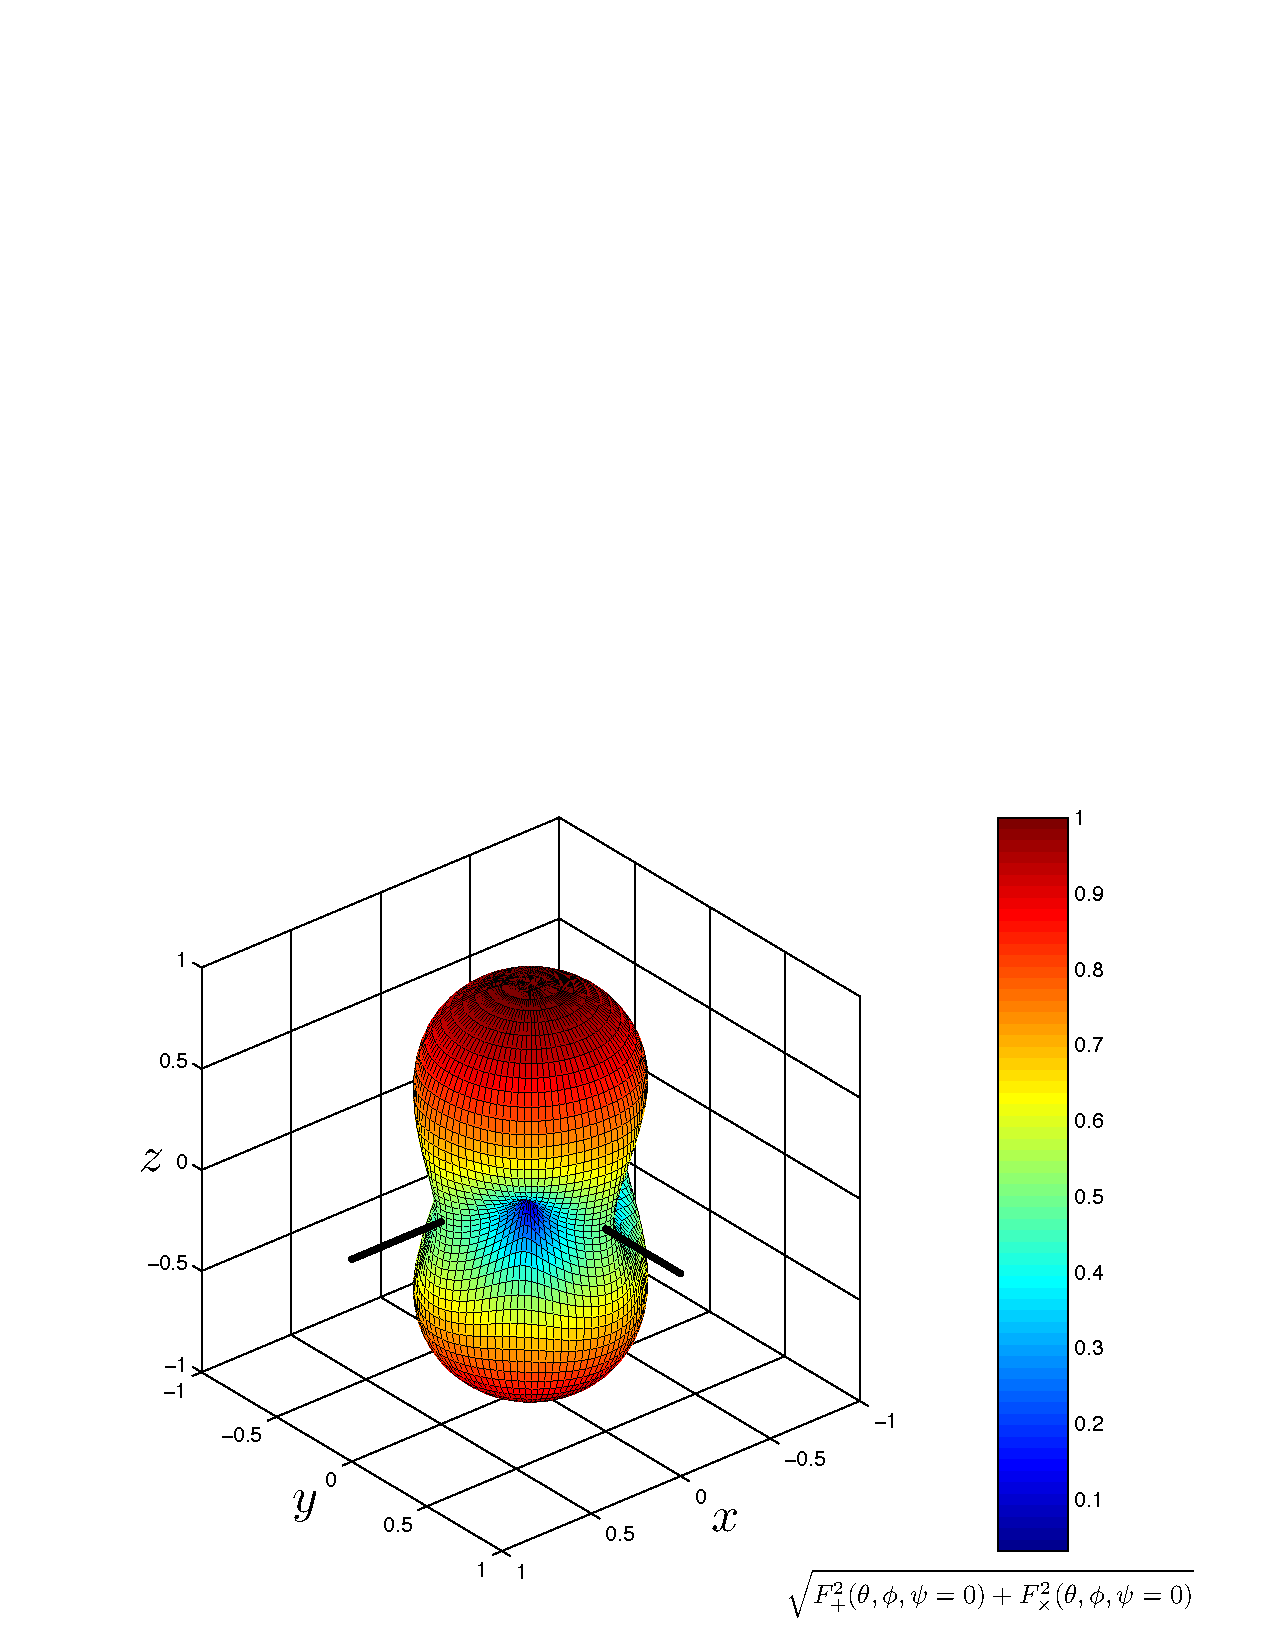
\includegraphics[width=6in]{figures/beampattern.pdf}
\caption{The antenna pattern of an \ac{IFO}. The arms of the interferometer are plotted for reference. Figure originally published in \cite{ref:Brown}.}
\end{figure}

\subsection{The LIGO and Virgo Interferometers}

The \ac{LSC} operates three \emph{\acp{IFO}}: two in at the \ac{LHO} in Hanford, Washington --- which we will denote H1 and H2 --- and one at the \ac{LLO} in Livingston, Lousianna, which we denote L1. The Virgo Collaboration operates one interferometer, which we denote V1, in Cascina, Italy. At root, these instruments run on the same basic principles as our toy interferometer described above. In practice, however, they are far more sophisticated, as they must account for a number of real-world problems; no description here would do them justice. Instead we note a few of their basic properties that are relevant to the later chapters of this thesis.

In the above section we found that the phase shift induced in the arms of the interferometer was proportional to the amplitude of the gravitational-wave, and to the length of the arm. This would suggest that the longer we make the arms, the more sensitive our instrument will be. However, if the light remains in the arm for a full cycle of the gravitational wave, any time dilation gained on the crest of the wave will be cancelled by the trough. We therefore wish the light to remain in the arms for $1/2$ the period of the \ac{GW}, as this will result in the maximum phase difference. If we are searching for waves with a frequency $\sim 100\,$Hz, this sets an optimal length for the arms to be:
\begin{equation}
L = \frac{\lambda}{4} = \frac{c}{2\fGW} = \frac{c}{200} \sim 1000\,\mathrm{km}
\end{equation}
This is a hopelessly large distance for a ground-based interferometer. The LIGO and Virgo \acp{IFO} deal with this difficulty by using \emph{Fabry-Perot cavities}.

Figure \ref{fig:fabry_perot} shows a schematic of a Fabry-Perot interferometer. By placing a semi-transparent mirror in the near-end of each arm --- referred to as the \emph{intermediate test masses} (ITMX and ITMY), to distinguish it from the \emph{end test masses} (ETMX and ETMY) --- a cavity is created. By keeping the length of the arms close the resonance of the light, the light bounces around for $~200$ more times \cite{ref:Brown} before exiting the arms. Thus the actual length of the arms can be $\mathcal{O}(1\,\mathrm{km})$ while the effective lenth will be $\mathcal{O}(10^3\,\mathrm{km})$. This results in the maximum detectable phase shift at $100\,$Hz. Both the \ac{LIGO} and Virgo interferometers are $\mathcal{O}(\mathrm{km})$: H1 and L1 are $4\,$km long, and V1 is $3\,$km. In \emph{initial} \ac{LIGO} H2 was $2\,$km, but this is planned to be expanded to $4\,$km for \emph{advanced} \ac{LIGO}.

For the Fabry-Perot cavity to work effectively, we need to keep the interferometer arms on resonance, or ``locked." This is done by a feedback look involving a series of servos. By monitoring motions of the mirrors through the output port (and other channels), the servos are actuated in order to keep the mirrors in lock. One of these channels monitors, and adjusts to, the differential arm length, or \verb|DARM_ERR|. Since a passing gravitational wave would show up as ocillations in \verb|DARM_ERR|, it is this channel that we monitor to search for \acp{GW}.

\begin{figure}[htbp]
\center
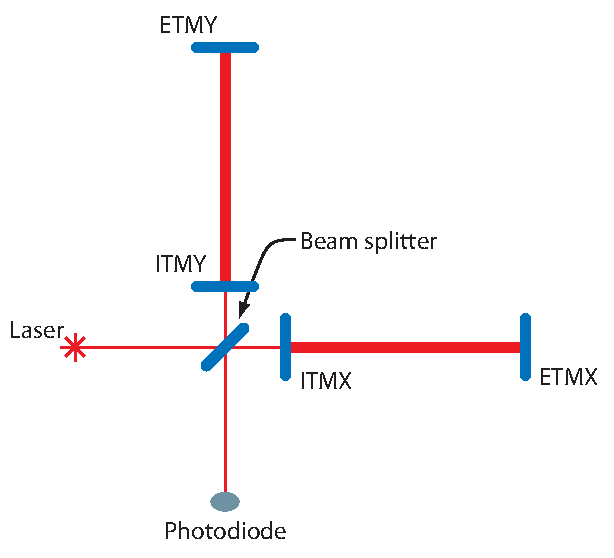
\includegraphics[height=3in]{figures/fabry-perot.pdf}
\caption{Schematic of an interferometer with a Fabry-Perot cavity.}
\label{fig:fabry_perot}
\end{figure}

Since gravitational waves are so weak, sources of noise are a major concern. We briefly note a few here:
\begin{itemize}
\item{\emph{Seismic Noise}: As the name suggests, this is noise due to ground motion. This motion can couple into the interferometer through the test masses' suspension system. To counteract it, a number of seismic isolation systems are put in place between the ground and the wires to which the test masses are attached. Seismic noise is primarily a problem at low-frequency. In initial \ac{LIGO}, the seismic ``wall" was at $\sim 40\,$Hz; in advanced \ac{LIGO} it is projected to be at $\sim 10\,$Hz. When analyzing \ac{LIGO} and Virgo data, we cut put a lower cut-off to the matched filter, $f_0$, at these frequencies.}
\item{\emph{Shot Noise}: This is the primary noise source at high ($~1\,$kHz) frequency. If we view the light in the interferometer from a quantum perspective, we recognize that we are limited by Poisson counting statistics of the photons. The error in the mean number of counts (which is the same as the intensity of the light) in some given amount of time goes as $1/\sqrt{N}$. Thus, as we consider higher frequencies, the error in our measurement of the light goes up. This suggests using a more powerful laser, which was done for enhanced \ac{LIGO}, and is planned for advanced \ac{LIGO}. However, more intense light will also cause higher radiation pressure on the mirrors --- which is noise source at lower frequencies --- and so these considerations must be balanced. Additionally, more intense light will heat up the mirrors, which causes greater ---}
\item{\emph{Thermal Noise}: This is due to the thermal vibrations in the mirrors and the wires from which the mirrors hang. This noise primarily affects frequencies in the $40\,$ to $200\,$Hz range.}
\end{itemize}
These, and other sources, add up to give the the amplitude spectral density, or ``noise curve" of the detectors. Figure \ref{fig:init_AdvASD} shows what the noise curves looked like for initial \ac{LIGO} and Virgo, and what they are expected to be for the advanced detector era.

All of these sources contribute to the \emph{stationary Gaussian} noise of the detectors. In addition, there are a number of environmental and instrumental transient sources, or ``glitches", for which we have no model. As discussed in the next few chapters, a major part of the \ac{CBC} data-analysis pipeline is mitigating the effect of these transient sources.

\begin{figure}[p]
\center
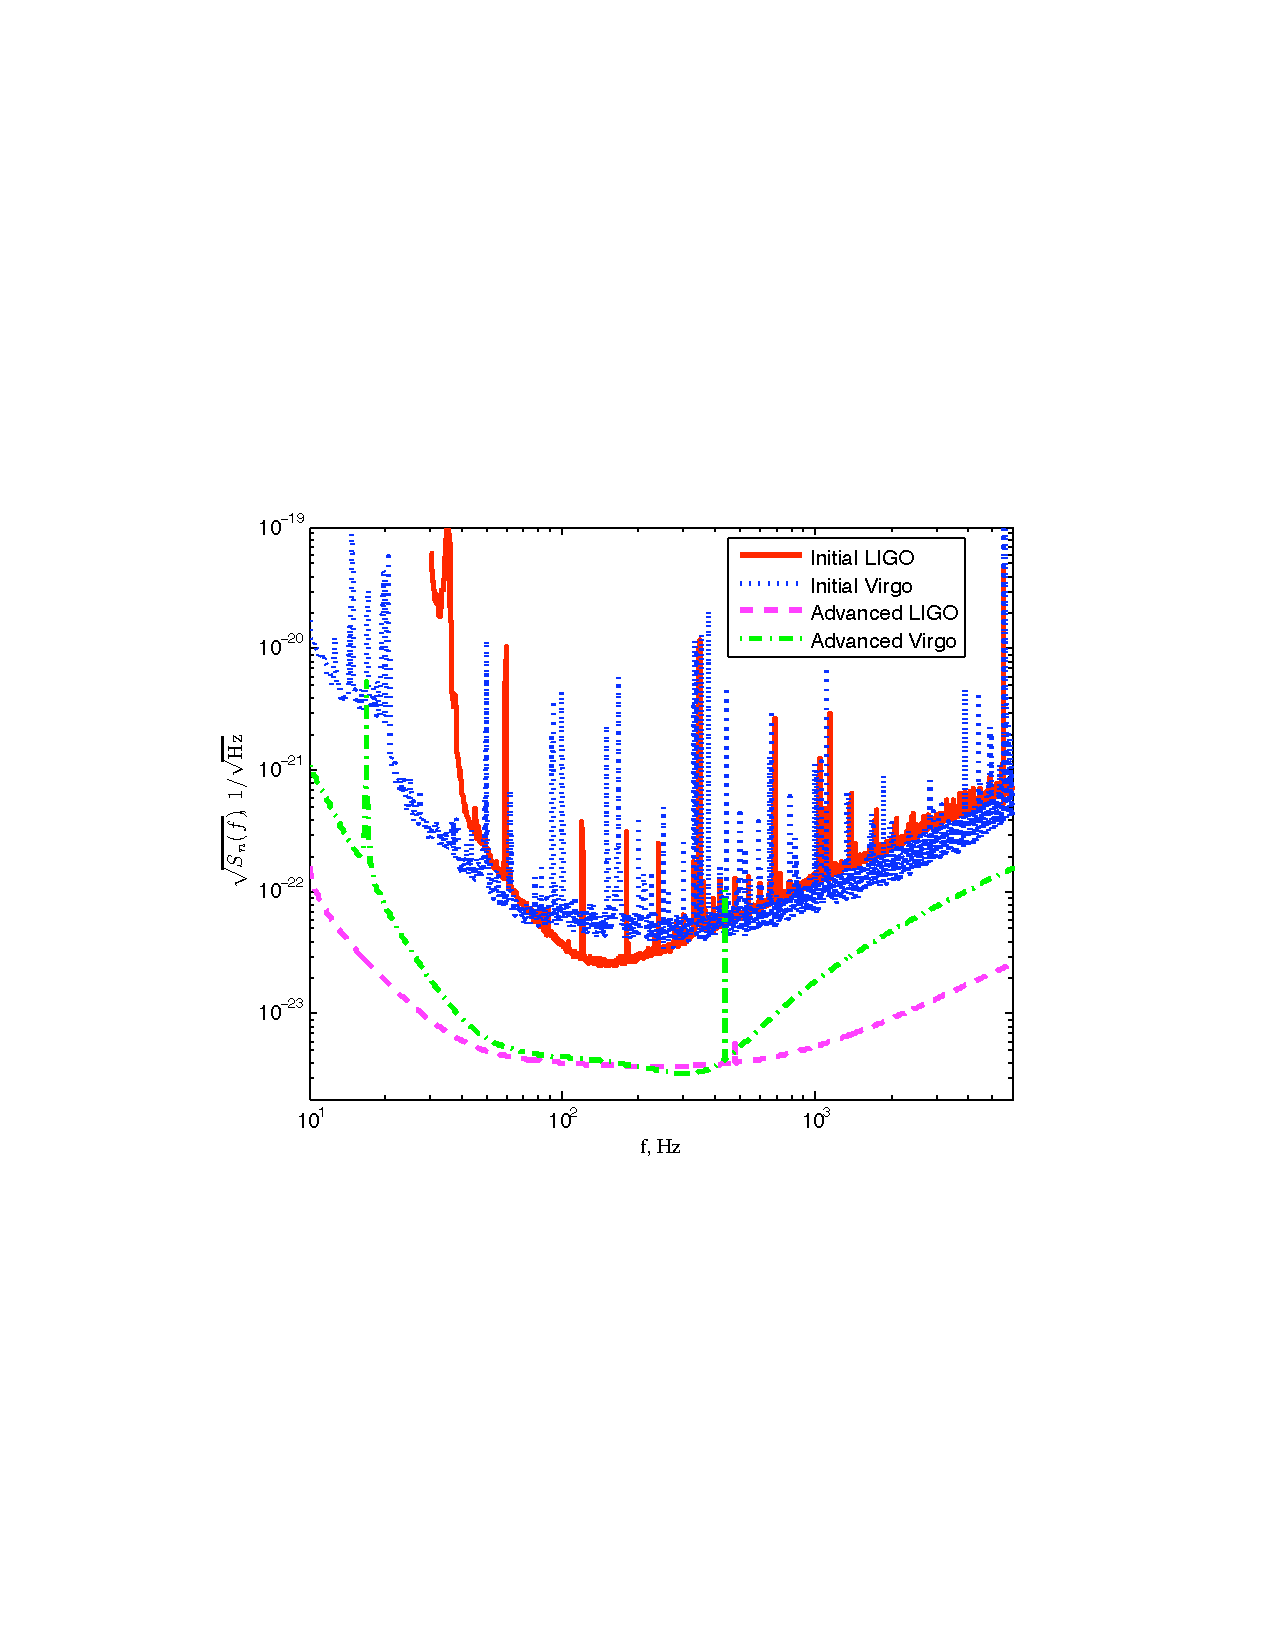
\includegraphics[width=6in]{figures/NoiseCurvesInitAdv.pdf}
\caption{Amplitude spectral densities of initial \ac{LIGO} and Virgo detectors. Shown also are the expected noise curves for advanced \ac{LIGO} and Virgo. Figure originally published in \cite{ref:rates}.}
\label{fig:init_AdvASD}
\end{figure}

\section{Astrophysical Sources of Gravitational Waves from Compact Binary Coalescence}

So far in our analysis we had to consider two objects with component masses on order of $\sim \Msun$ orbiting at frequencies of $\sim 10^2\,$Hz to obtain realistically measureable \acp{GW}. While such systems may seem realistically implausible, it turns out these systems do naturally occur in the universe. Of interest to us are binary-neutron star systems, binary black hole systems and neutron-star black-hole binaries.

Table \ref{tab:bns_bbh_rates} gives estimated rates of \ac{BNS}, \ac{NSBH}, and \ac{BBH} coalescence in the universe. The component masses used in the estimates are $1.4/1.4\Msun$, $1.4/10.0\Msun$, and $10.0/10.0\Msun$. The uncertainty in these estimates are large, varying by as much as two orders of magnitude. This is due to the small sample size of observed systems, and from uncertainties in the population synthesis models on which some rates are based. Rates of systems involving black holes are perhaps the most uncertain, since no black hole has (or can) be directly observed by telescopes.\footnote{Being able to directly detect black holes, and measure properties of their curvature, is a major advantage of \ac{GW} detectors.} We can be more confident about \ac{BNS} rates, however, as these have been directly observed. Of note is the Hulse-Taylor pulsar, which was shown to be losing energy at the rate expected from \ac{GW} emission. The separation distance between the system's constituent neutron stars is such that they will not coalesce for another $300\,$ million years, however.

Using the \ac{LIGO} and Virgo noise \ac{PSD} we can estimate the expected rate of detections in a year of data at a given detection threshold (how this is done is detailed in the next Chapter). Table \ref{tab:detection_rates} shows the estimated rate in initial \ac{LIGO} is and what it is expected to be for advanced \ac{LIGO}. As we can see, the rates in initial \ac{LIGO} are all less than one per year, even on the optimistic end. For advanced \ac{LIGO}, however, we see that the expected detection rates are on order of $\sim 10$ per year. We expect advanced \ac{LIGO} to have a range that is $\sim10$ times that of initial \ac{LIGO}. Thus we get factor of $\sim1000$ increase in sensitive volume.

The advanced \ac{LIGO} rates are based on the projected sensitivity of the detector and on our ability to detect a \ac{GW} event at a signal-to-noise ratio of 8. (See the next chapter for a discussion of signal-to-noise ratio.) Since initial \ac{LIGO} has already happened, we can base our rates on what we observed. If we do not detect a \ac{GW} event (to some confidence level) we can use the time searched and the sensitivity of the instrument to set an upper-limit on the rate of \acp{CBC} in the universe. This is done using the \emph{loudest-event statistic} method \cite{ref:uls}. After performing a search, we calculate the relative probablility that the loudest event was due to a \ac{GW} as compared to the probabliity it was due to noise, or background. We then calculate the efficiency of the \acp{IFO} at detecting signals with the same value of the ranking statistic\footnote{To rank triggers we use the inverse false alarm rate, or IFAR. See chapters \ref{ch:far}, \ref{ch:ihope_pipeline}, and \ref{ch:s5_results} for details.} as the loudest event. This is done by injecting fake signals, or ``software injections" into the data then checking how well they are recovered by our data-analysis pipeline. Performing a Monte Carlo integral over all of the injections gives us an estimate of the detector's efficiency. Since we know the effective distance of the injections, we can put the efficiency in terms of distance. From that, we get the sensitive volume of the universe the search was sensitive to.\footnote{When computing the sensitive volume we must take into account the expected astophysical distribution of sources. In initial \ac{S5} this was done by using a galaxy cataloge. In \ac{S6}, the range of the detectors is large enough that we can assume the sources are uniformly distributed across the sky, which allows us to simply use the range.} Combining this with the observation time, we get a rate upper limit of:
\begin{equation}
\label{eqn:rate_ul}
\mathcal{R}_{90\%} = \frac{\beta}{VT}
\end{equation}
where $V$ is the sensitive volume and $T$ is the observation time; the rate is computed to the $90\%$ confidence level. The factor $\beta$ depends on the likelihood that the loudest event was a signal. As the likelihood goes to zero (i.e., the probablity is low that the data contains a \ac{GW}), then $\beta \rightarrow 2.303$ at the $90\%$ confidence level. As the likelihood goes to infinity (i.e., the probability is high that the data contains a \ac{GW}) $\beta \rightarrow 3.9$ \cite{ref:uls}.

In Chapter \ref{ch:s5_results} we present upper limits calculated from a six-month long search of \ac{S5} data using the loudest-event statistic method. For more details on the loudest-event statistic method see \cite{ref:uls}. For more details on how the rates presented in Table \ref{tab:bns_bbh_rates} were calculated, see \cite{ref:ratesPaper} and the papers cited therein.

\begin{table}[p]
\center
\begin{tabular}{ c | c | c | c }
\hline
Source  &   $R_{\mathrm{low}}~(\Mpc^{-3}\mathrm{Myr}^{-1})$    &   $R_{\mathrm{best}}~(\Mpc^{-3}\mathrm{Myr}^{-1})$   &   $R_{\mathrm{high}}~(\Mpc^{-3}\mathrm{Myr}^{-1})$ \\
\hline
\ac{BNS}    & 0.01  &   1   &   10 \\
\ac{NSBH}   & $6\times10^{-4}$   &   0.03    & 1 \\
\ac{BBH}    & $1\times10^{-4}$  &   0.005   &   0.3 \\
\hline
\end{tabular}
\caption{Estimated rates of \ac{BNS}, \ac{NSBH}, and \ac{BBH} coalescence in the universe. $R_{\mathrm{best}}$ indicates best estimate; ``low" and ``high" indicate pesimistic and optimistic rates, respectively. The component masses used in the estimates are $1.4/1.4\Msun$ for \ac{BNS}, $1.4/10.0\Msun$ for \ac{NSBH}, and $10.0/10.0\Msun$ for \ac{BBH}. For details on how these numbers were derived, see \cite{ref:rates}.}
\label{tab:bns_bbh_rates}
\end{table}

\begin{table}[p]
\center
\begin{tabular}{ c | c | c | c | c }
\hline
Era &   Source  &   $\dot{N}_{\mathrm{low}}~(\yr^{-1})$    &   $\dot{N}_{\mathrm{best}}~(\yr^{-1})$   &   $\dot{N}_{\mathrm{high}}~(\yr^{-1})$ \\
\hline
\multirow{3}{*}{Initial}    &   \ac{BNS}    & $2\times 10^{-4}$ & 0.02    &   0.2 \\
    &   \ac{NSBH} & $7\times10^{-5}$    &   $0.004$ &   $0.1$ \\
    &   \ac{BBH}  & $2\times10^{-4}$    &   $0.007$ &   $0.5$ \\
\hline
\multirow{3}{*}{Advanced}    &  \ac{BNS}    &  0.4    &   40  &   400 \\
    &   \ac{NSBH}   &   0.2 &   10  &   300 \\
    &   \ac{BBH}    &   0.4 &   20  &   1000 \\
\hline
\end{tabular}
\caption{Estimated detection rates in initial and advanced \ac{LIGO}. The component masses used in the estimates are $1.4/1.4\Msun$ for \ac{BNS}, $1.4/10.0\Msun$ for \ac{NSBH}, and $10.0/10.0\Msun$ for \ac{BBH}. For details on how these numbers were derived, see \cite{ref:rates}.}
\label{tab:detection_rates}
\end{table}

%By computing upper-limits we can compare our results to astrophysically expected event rates. To date, no \acp{GW} have been detected. However, based on our current sensitivity, the resulting upper limits are still approximately an order of magnitude higher then astrophysical best estimates. When advanced \ac{LIGO} comes online, however, we  

